\chapter{$v_2(\pt)$ with Different $\Psi_2$ Weighting}	% *NOT* \OnePageChapter
\label{sec:appendix}
In this appendix, we show the $v_2(\pt)$ measurement with the FVTXS and BBCS event plane with various corrections which are described in Chapter 4. We show $v_2(\pt)$ for each layer of the FVTX and each ring of the BBC separately. 

\begin{figure}
\centering
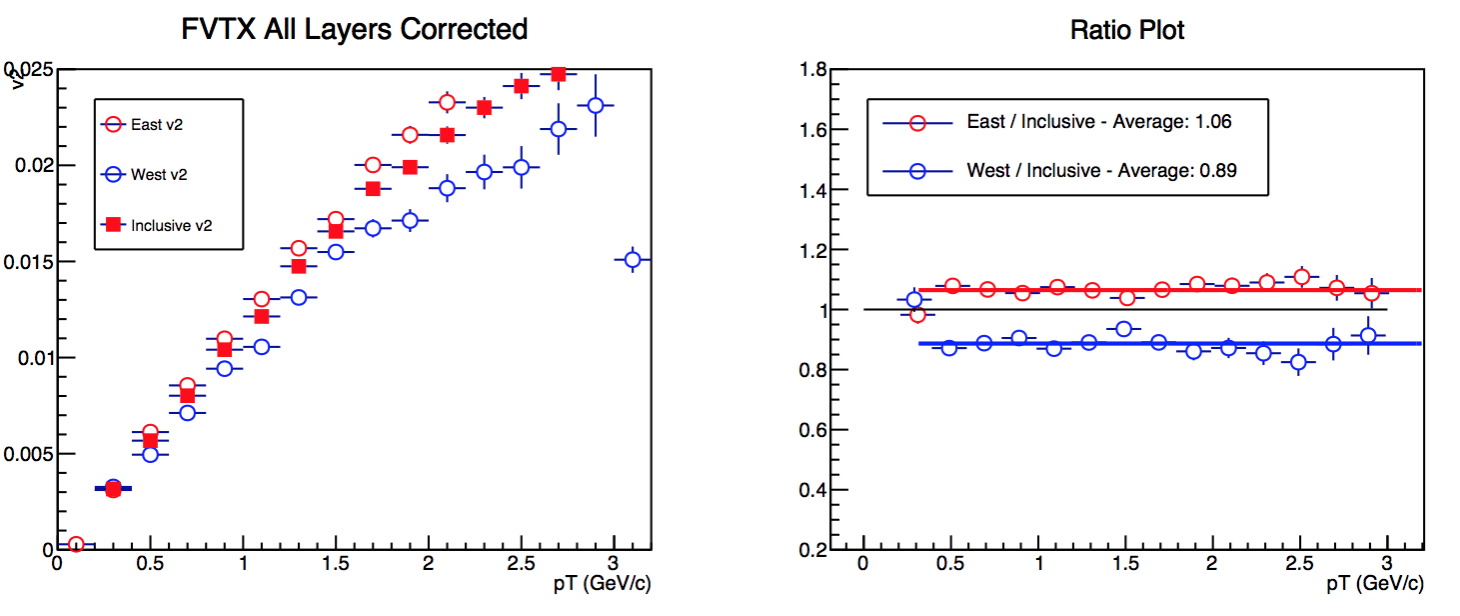
\includegraphics[width=0.65\linewidth]{figs/fvtx_all_default.png}
\caption{FVTXS event plane measurement with default correction and FVTX layers 1, 2, and 4 of $v_{2}(\pt)$ with the  for the \pau \sqsn = 200 GeV (left) and the ratio of the east and west $v_2$ measurements to the inclusive $v_2$ (right).}
\end{figure}

\begin{figure}
\centering
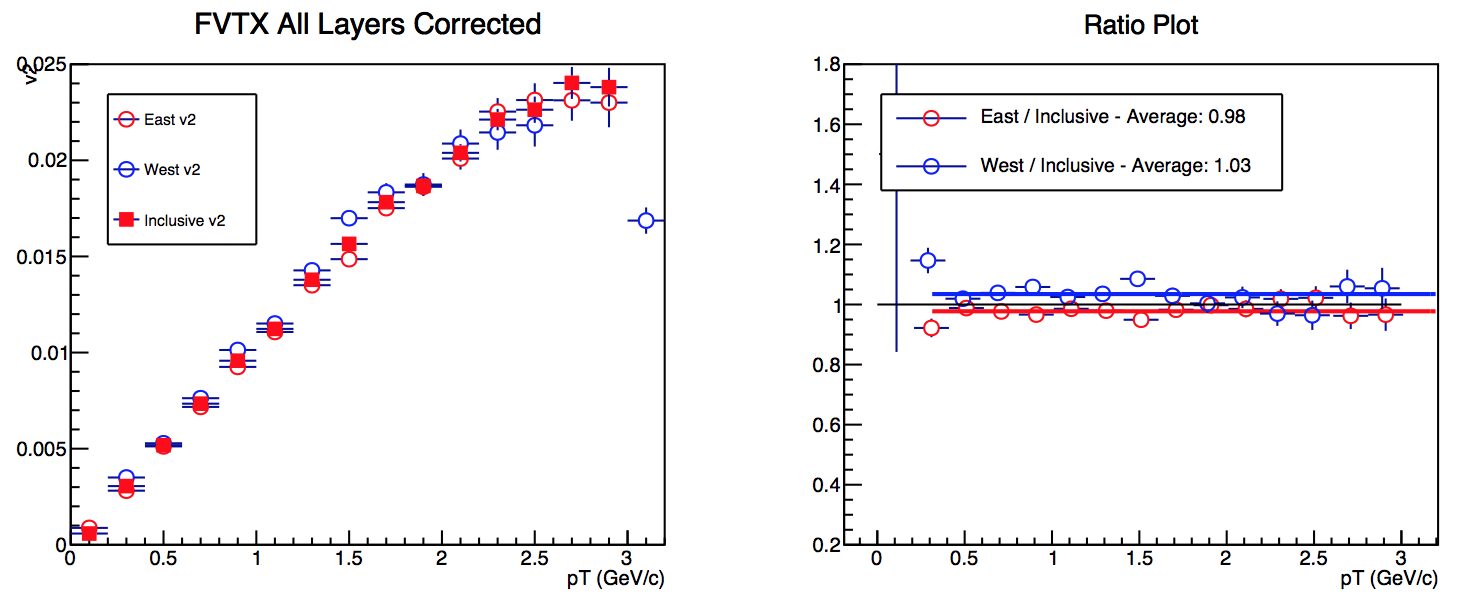
\includegraphics[width=0.65\linewidth]{figs/fvtx_all_data.png}
\caption{FVTXS event plane measurement with inverse $\phi$ weighting and FVTX layers 1, 2, and 4 of $v_{2}(\pt)$ with the  for the \pau \sqsn = 200 GeV (left) and the ratio of the east and west $v_2$ measurements to the inclusive $v_2$ (right).}
\end{figure}

\begin{figure}
\centering
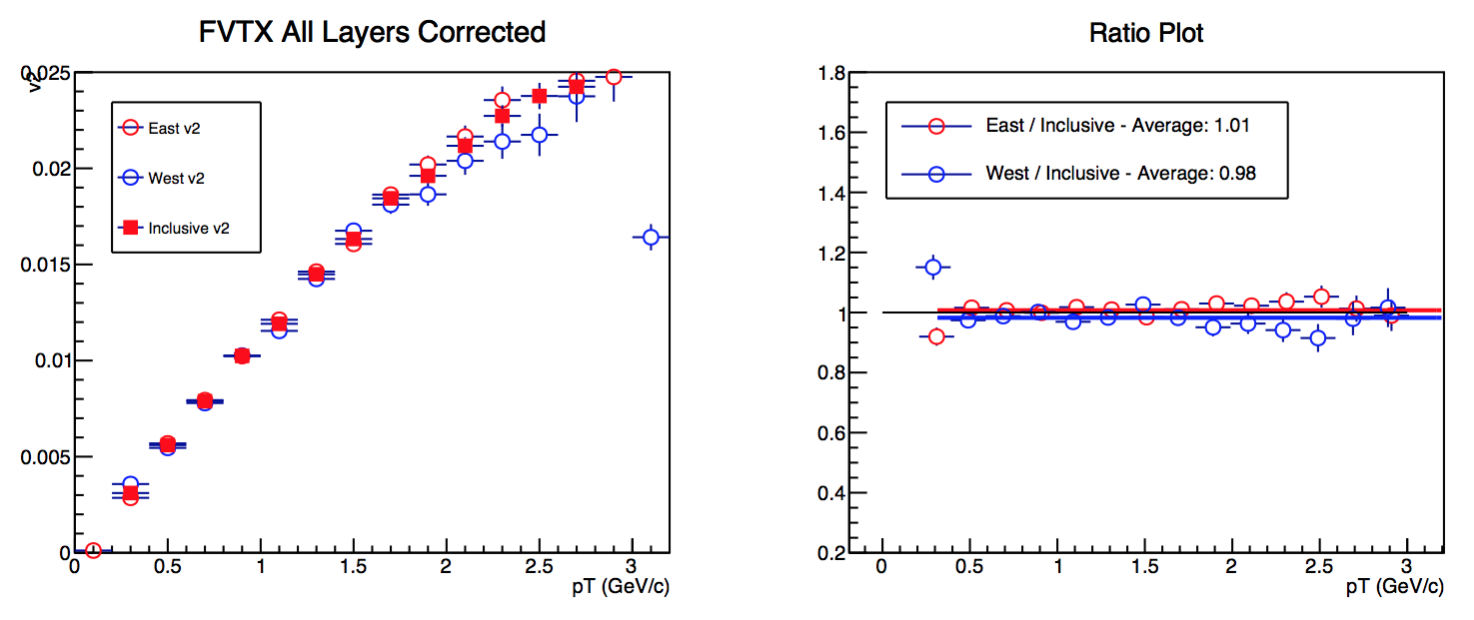
\includegraphics[width=0.65\linewidth]{figs/fvtx_all_analytic.png}
\caption{FVTXS event plane measurement with analytic weighting and a 20\% cut and FVTX layers 1, 2, and 4 of $v_{2}(\pt)$ with the  for the \pau \sqsn = 200 GeV (left) and the ratio of the east and west $v_2$ measurements to the inclusive $v_2$ (right).}
\end{figure}

\begin{figure}
\centering
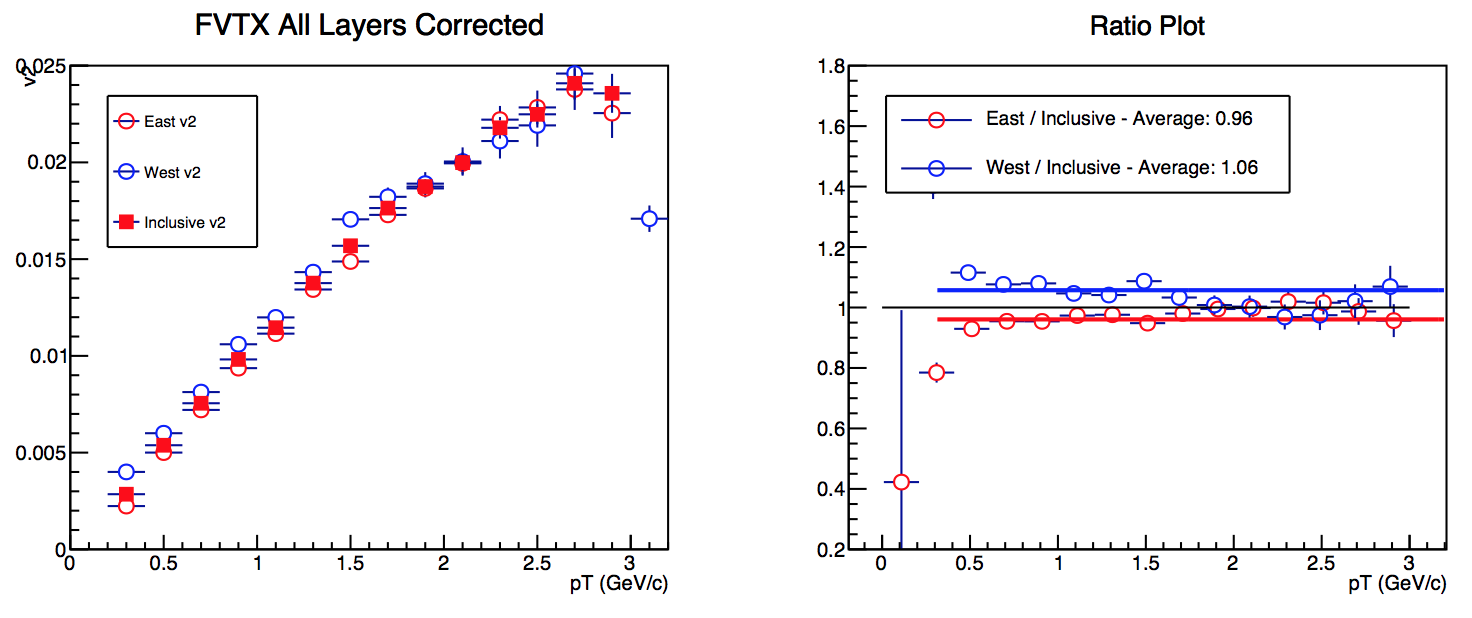
\includegraphics[width=0.65\linewidth]{figs/fvtx_all_data_cut.png}
\caption{FVTXS event plane measurement with inverse $\phi$ weighting and a 20\% cut and FVTX layers 1, 2, and 4 of $v_{2}(\pt)$ with the  for the \pau \sqsn = 200 GeV (left) and the ratio of the east and west $v_2$ measurements to the inclusive $v_2$ (right).}
\end{figure}

\begin{figure}
\centering
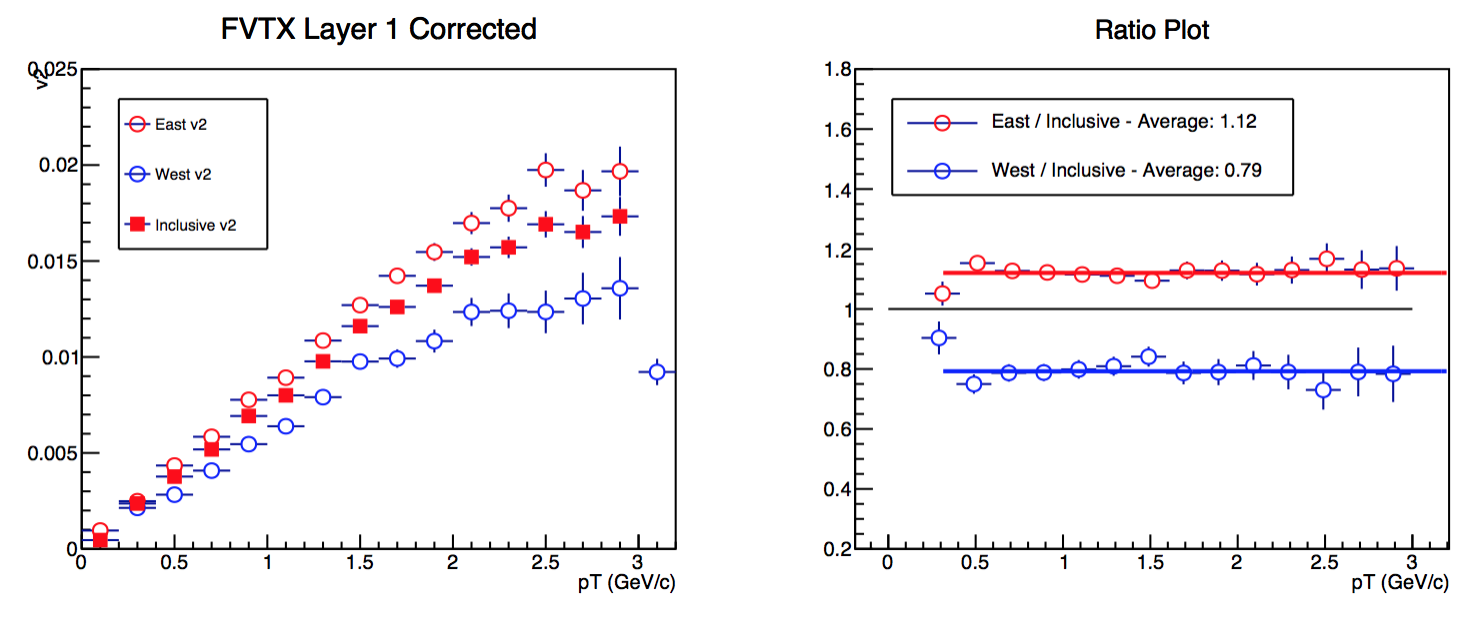
\includegraphics[width=0.65\linewidth]{figs/fvtx_1_default.png}
\caption{FVTXS event plane measurement with default correction and FVTX layer 1 of $v_{2}(\pt)$ with the  for the \pau \sqsn = 200 GeV (left) and the ratio of the east and west $v_2$ measurements to the inclusive $v_2$ (right).}
\end{figure}

\begin{figure}
\centering
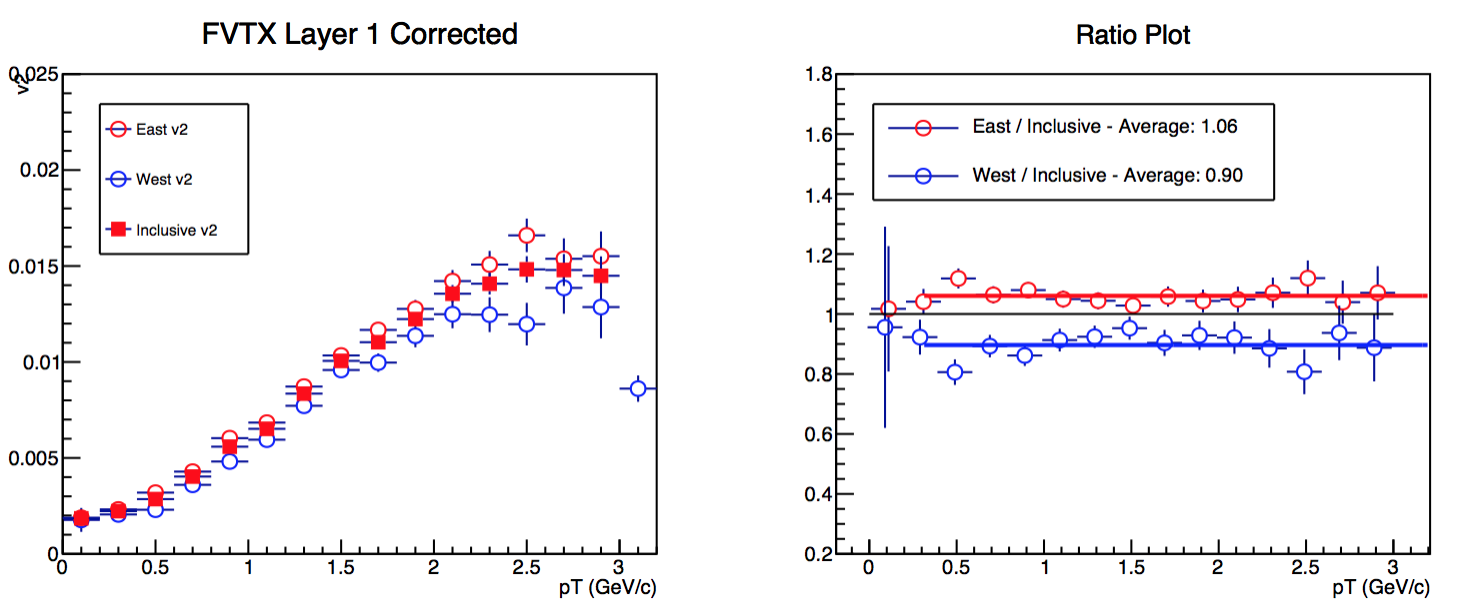
\includegraphics[width=0.65\linewidth]{figs/fvtx_1_data.png}
\caption{FVTXS event plane measurement with inverse $\phi$ weighting and FVTX layer 1 of $v_{2}(\pt)$ with the  for the \pau \sqsn = 200 GeV (left) and the ratio of the east and west $v_2$ measurements to the inclusive $v_2$ (right).}
\end{figure}

\begin{figure}

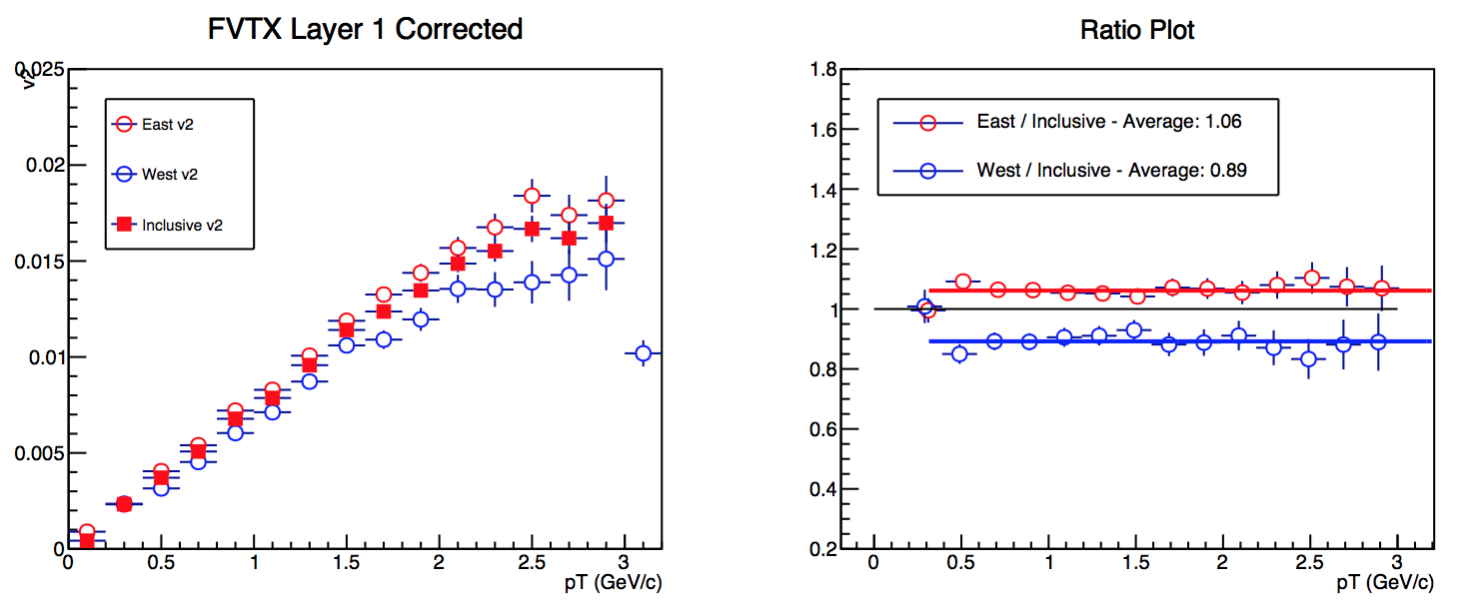
\includegraphics[width=0.65\linewidth]{figs/fvtx_1_analytic.png}
\caption{FVTXS event plane measurement with analytic weighting and a 20\% cut and FVTX layer 1 of $v_{2}(\pt)$ with the  for the \pau \sqsn = 200 GeV (left) and the ratio of the east and west $v_2$ measurements to the inclusive $v_2$ (right).}
\end{figure}

\begin{figure}

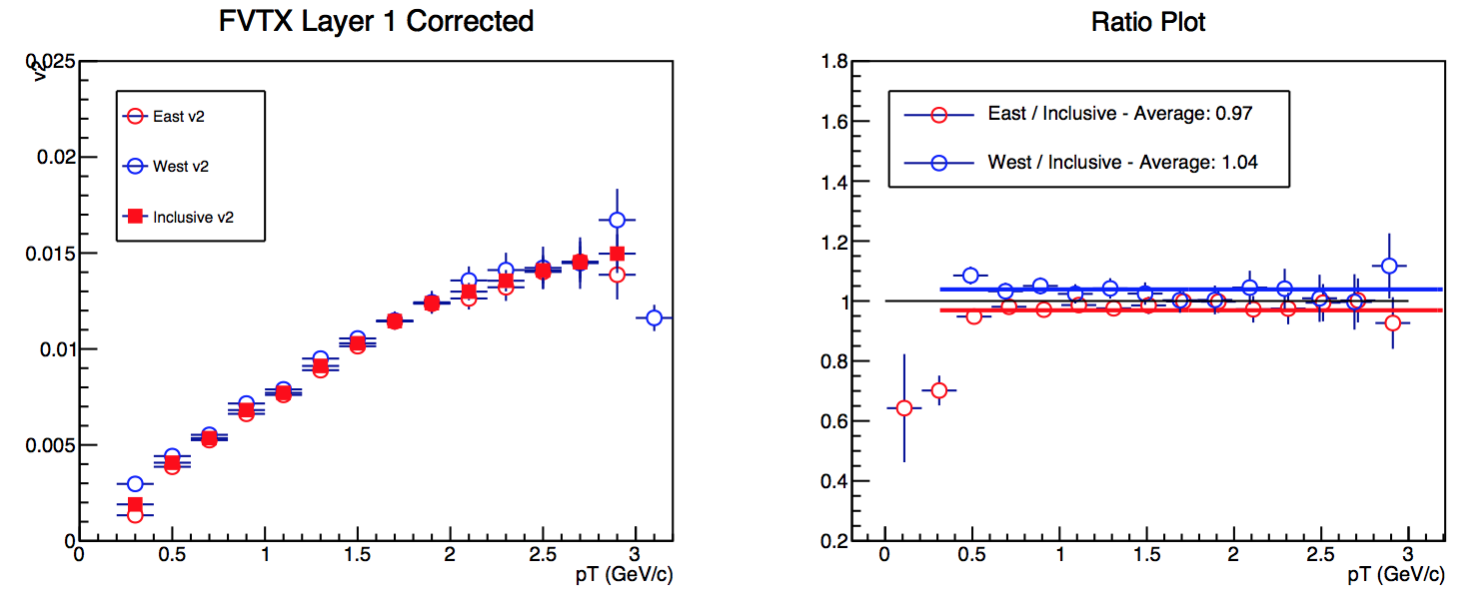
\includegraphics[width=0.65\linewidth]{figs/fvtx_1_data_cut.png}
\caption{FVTXS event plane measurement with inverse $\phi$ weighting and a 20\% cut and FVTX layer 1 of $v_{2}(\pt)$ with the  for the \pau \sqsn = 200 GeV (left) and the ratio of the east and west $v_2$ measurements to the inclusive $v_2$ (right).}
\end{figure}

\begin{figure}

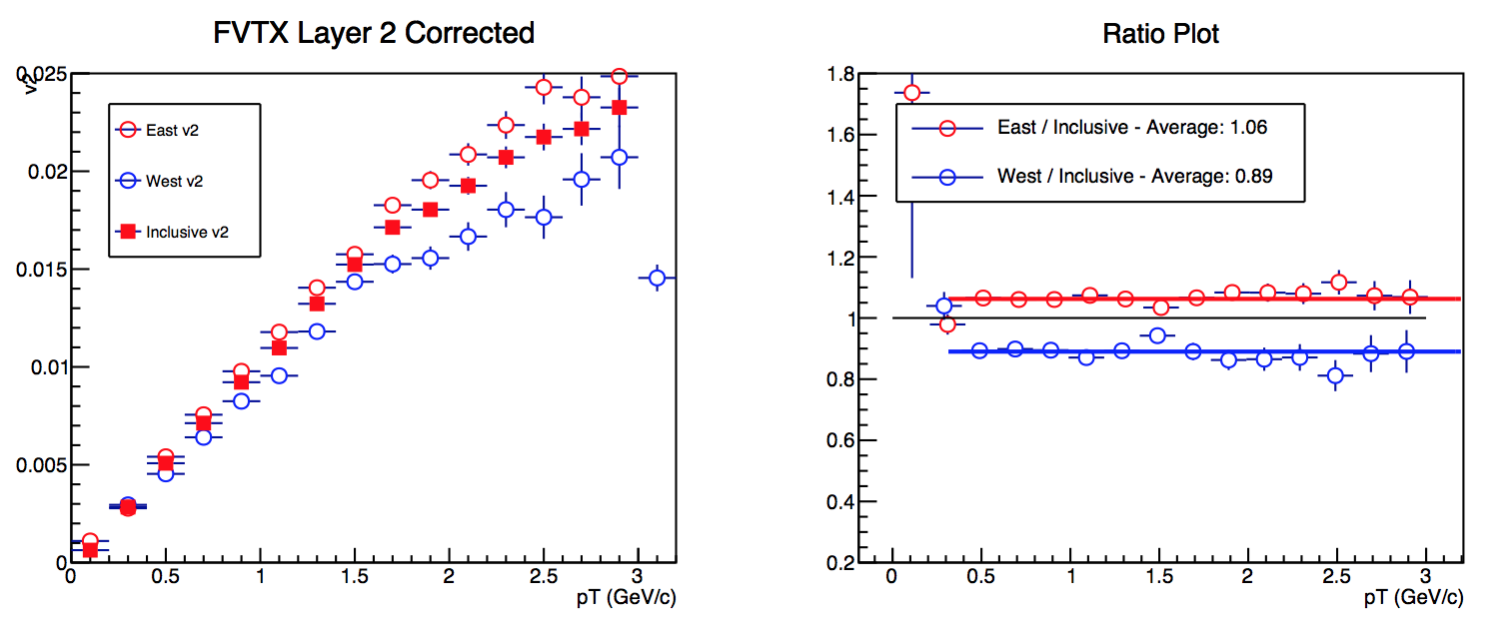
\includegraphics[width=0.65\linewidth]{figs/fvtx_2_default.png}
\caption{FVTXS event plane measurement with default correction and FVTX layer 2 of $v_{2}(\pt)$ with the  for the \pau \sqsn = 200 GeV (left) and the ratio of the east and west $v_2$ measurements to the inclusive $v_2$ (right).}
\end{figure}

\begin{figure}
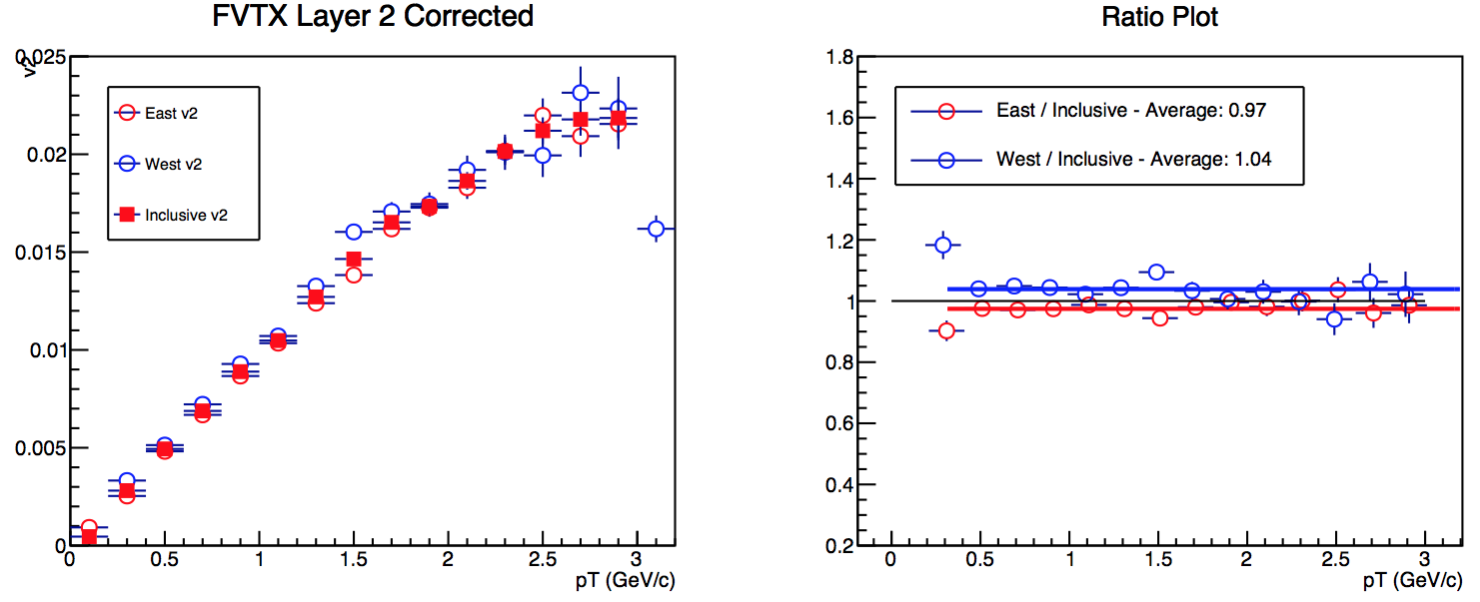
\includegraphics[width=0.65\linewidth]{figs/fvtx_2_data.png}
\caption{FVTXS event plane measurement with inverse $\phi$ weighting and FVTX layer 2 of $v_{2}(\pt)$ with the  for the \pau \sqsn = 200 GeV (left) and the ratio of the east and west $v_2$ measurements to the inclusive $v_2$ (right).}
\end{figure}

\begin{figure}
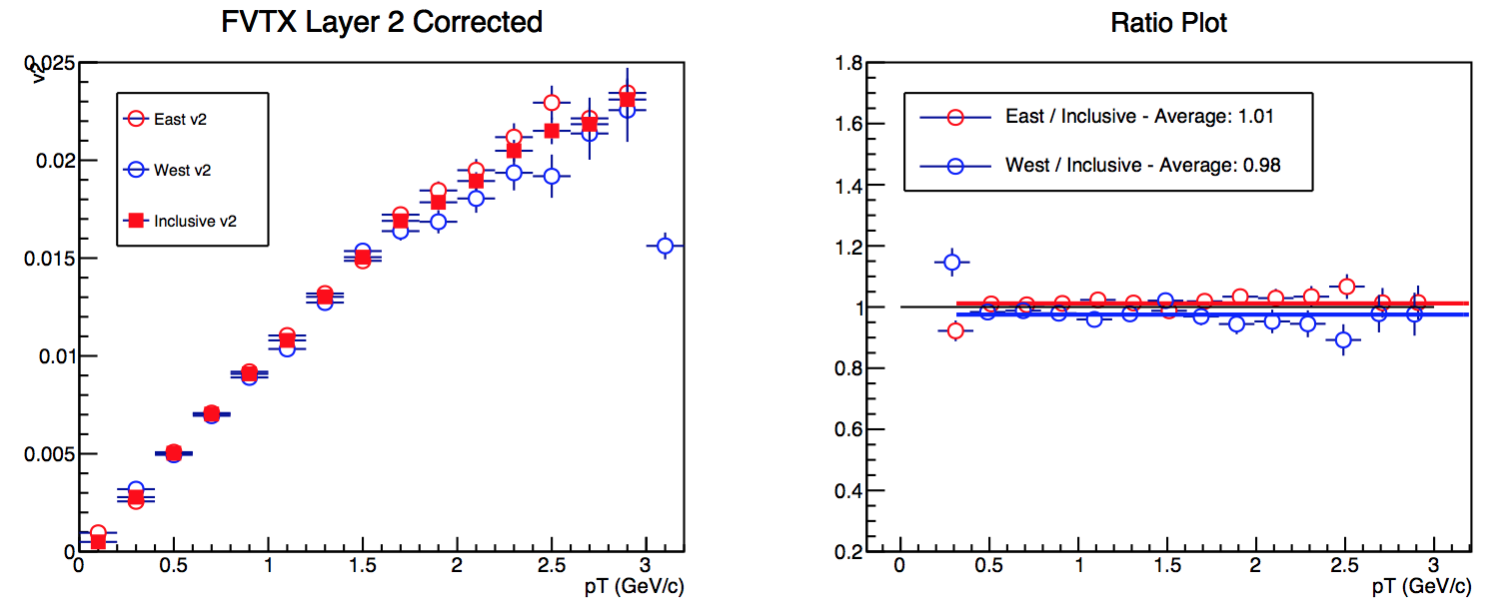
\includegraphics[width=0.65\linewidth]{figs/fvtx_2_analytic.png}
\caption{FVTXS event plane measurement with analytic weighting and a 20\% cut and FVTX layer 2 of $v_{2}(\pt)$ with the  for the \pau \sqsn = 200 GeV (left) and the ratio of the east and west $v_2$ measurements to the inclusive $v_2$ (right).}
\end{figure}

\begin{figure}
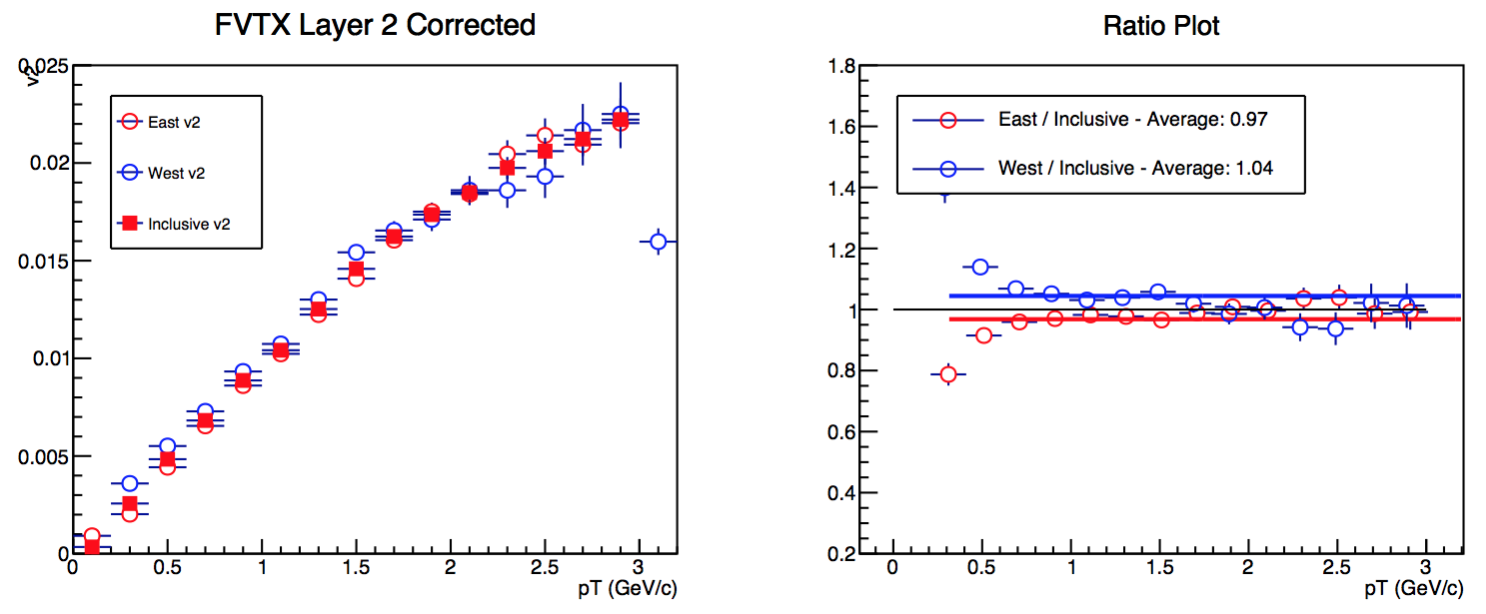
\includegraphics[width=0.65\linewidth]{figs/fvtx_2_data_cut.png}
\caption{FVTXS event plane measurement with inverse $\phi$ weighting and a 20\% cut and FVTX layer 2 of $v_{2}(\pt)$ with the  for the \pau \sqsn = 200 GeV (left) and the ratio of the east and west $v_2$ measurements to the inclusive $v_2$ (right).}
\end{figure}

\begin{figure}
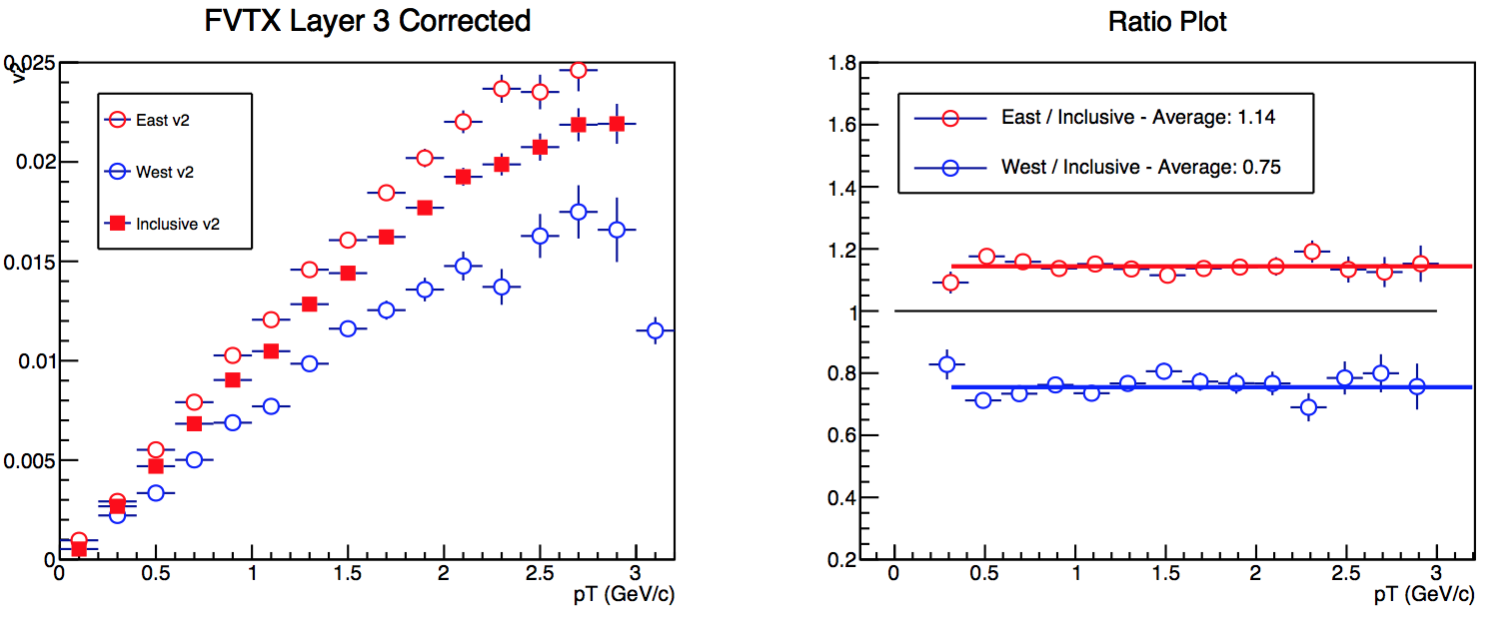
\includegraphics[width=0.65\linewidth]{figs/fvtx_3_default.png}
\caption{FVTXS event plane measurement with default correction and FVTX layer 3 of $v_{2}(\pt)$ with the  for the \pau \sqsn = 200 GeV (left) and the ratio of the east and west $v_2$ measurements to the inclusive $v_2$ (right).}
\end{figure}

\begin{figure}
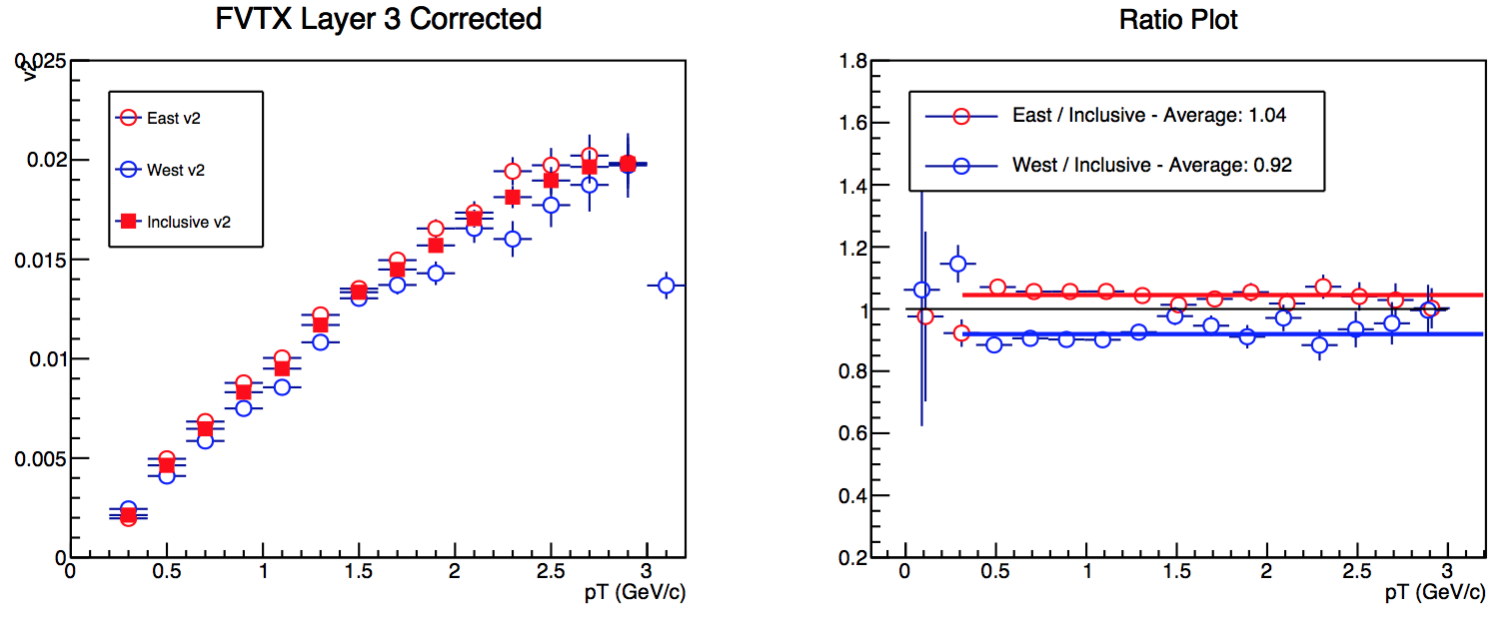
\includegraphics[width=0.65\linewidth]{figs/fvtx_3_data.png}
\caption{FVTXS event plane measurement with inverse $\phi$ weighting and FVTX layer 3 of $v_{2}(\pt)$ with the  for the \pau \sqsn = 200 GeV (left) and the ratio of the east and west $v_2$ measurements to the inclusive $v_2$ (right).}
\end{figure}

\begin{figure}
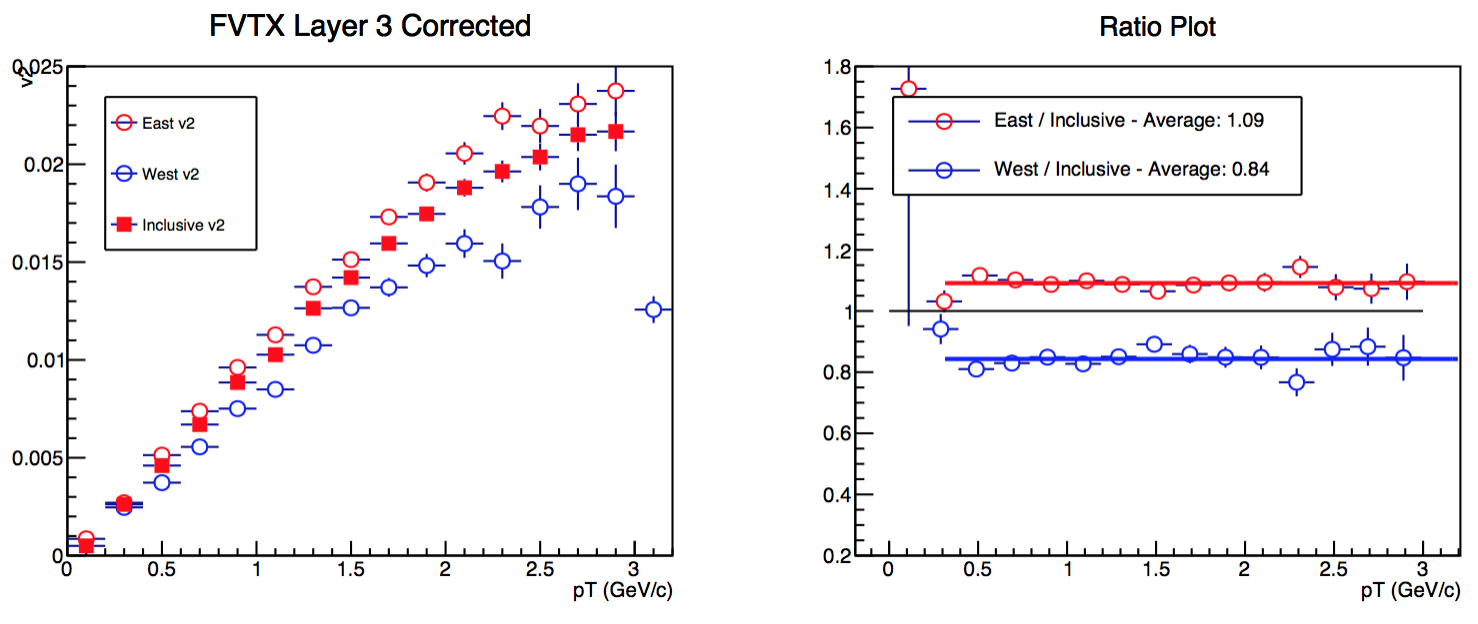
\includegraphics[width=0.65\linewidth]{figs/fvtx_3_analytic.png}
\caption{FVTXS event plane measurement with analytic weighting and a 20\% cut and FVTX layer 3 of $v_{2}(\pt)$ with the  for the \pau \sqsn = 200 GeV (left) and the ratio of the east and west $v_2$ measurements to the inclusive $v_2$ (right).}
\end{figure}
\clearpage
\begin{figure}

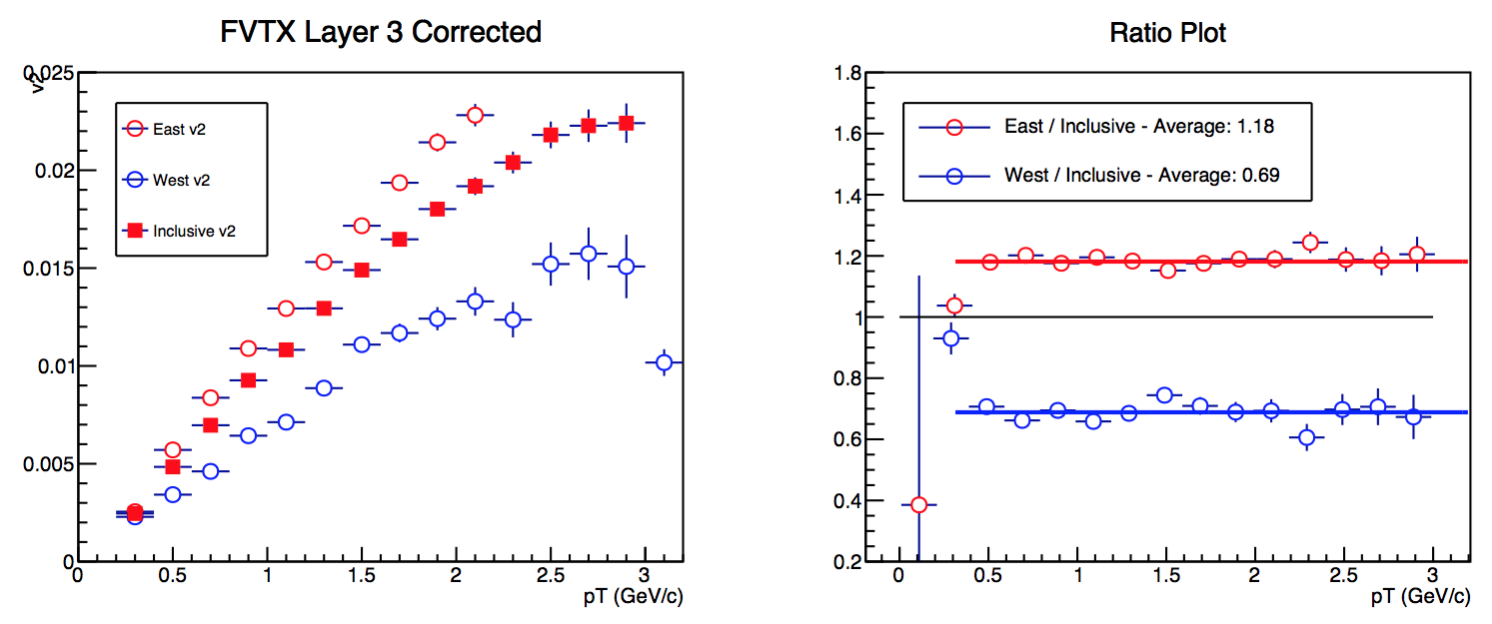
\includegraphics[width=0.65\linewidth]{figs/fvtx_3_data_cut.png}
\caption{FVTXS event plane measurement with inverse $\phi$ weighting and a 20\% cut and FVTX layer 3 of $v_{2}(\pt)$ with the  for the \pau \sqsn = 200 GeV (left) and the ratio of the east and west $v_2$ measurements to the inclusive $v_2$ (right).}
\end{figure}

\begin{figure}

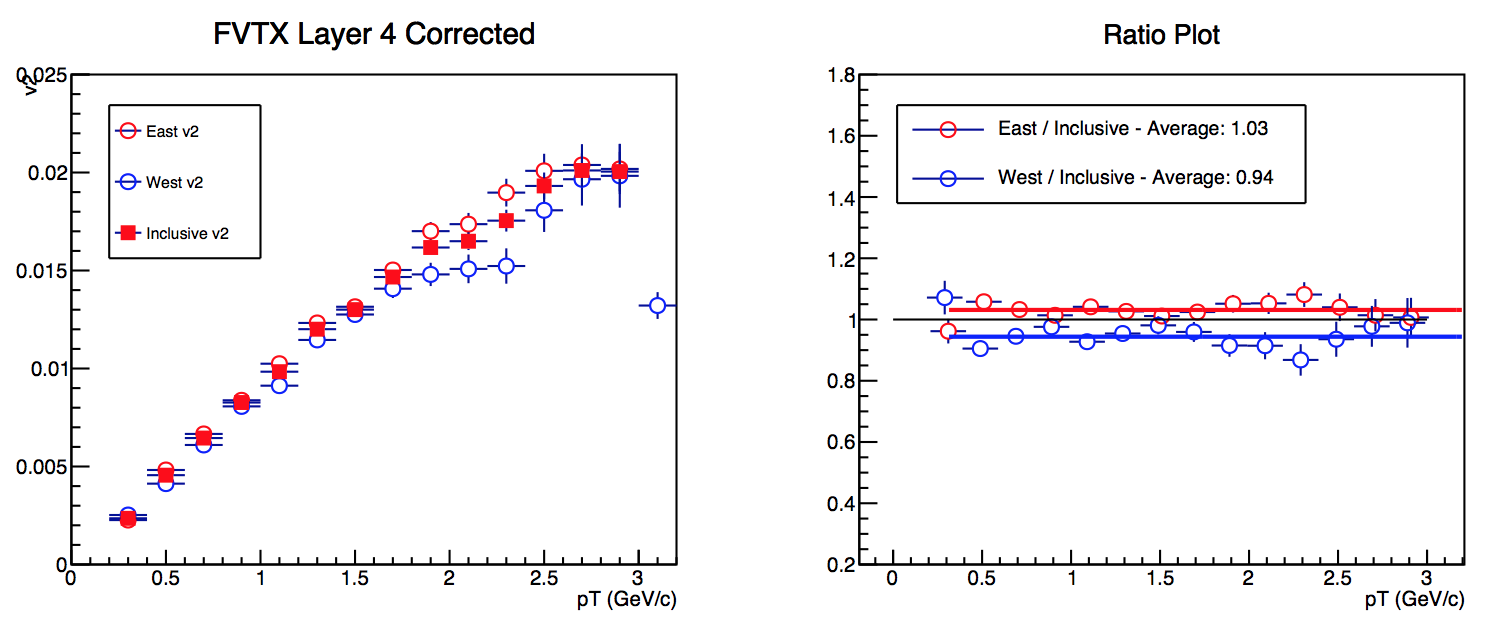
\includegraphics[width=0.65\linewidth]{figs/fvtx_4_default.png}
\caption{FVTXS event plane measurement with default correction and FVTX layer 4 of $v_{2}(\pt)$ with the  for the \pau \sqsn = 200 GeV (left) and the ratio of the east and west $v_2$ measurements to the inclusive $v_2$ (right).}
\end{figure}

\begin{figure}

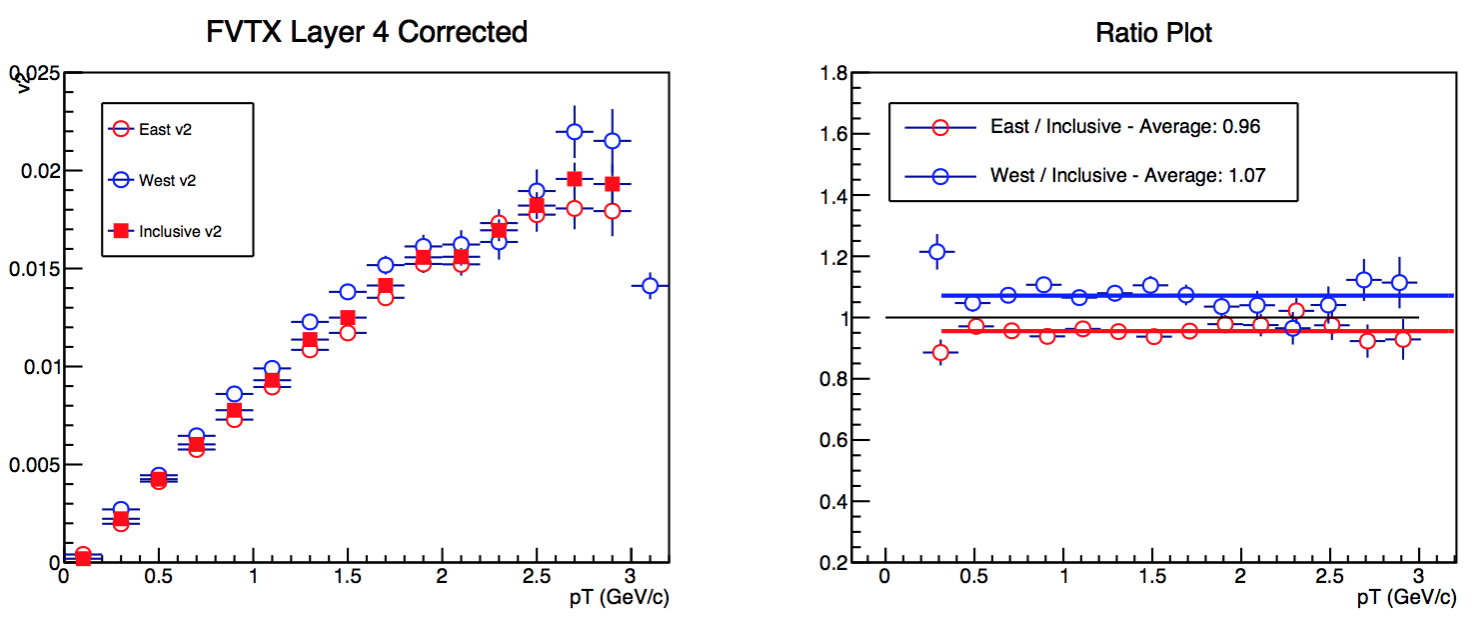
\includegraphics[width=0.65\linewidth]{figs/fvtx_4_data.png}
\caption{FVTXS event plane measurement with inverse $\phi$ weighting and FVTX layer 4 of $v_{2}(\pt)$ with the  for the \pau \sqsn = 200 GeV (left) and the ratio of the east and west $v_2$ measurements to the inclusive $v_2$ (right).}
\end{figure}

\begin{figure}

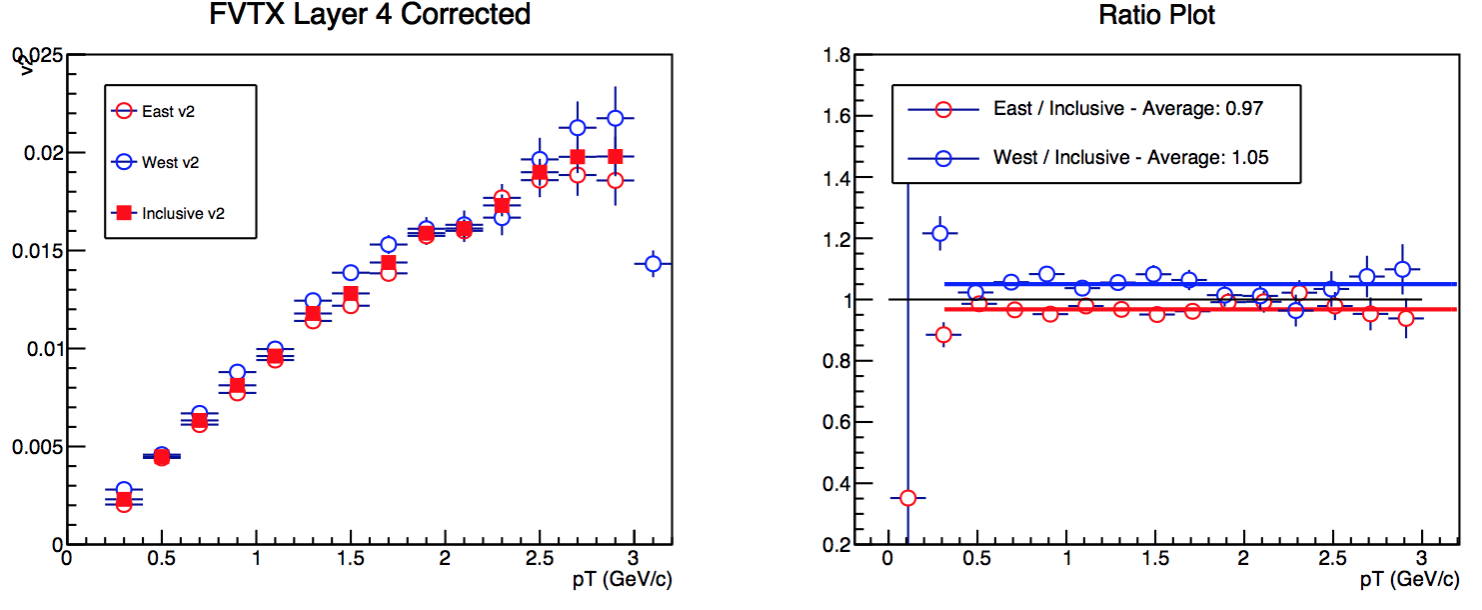
\includegraphics[width=0.65\linewidth]{figs/fvtx_4_analytic.png}
\caption{FVTXS event plane measurement with analytic weighting and a 20\% cut and FVTX layer 4 of $v_{2}(\pt)$ with the  for the \pau \sqsn = 200 GeV (left) and the ratio of the east and west $v_2$ measurements to the inclusive $v_2$ (right).}
\end{figure}

\begin{figure}

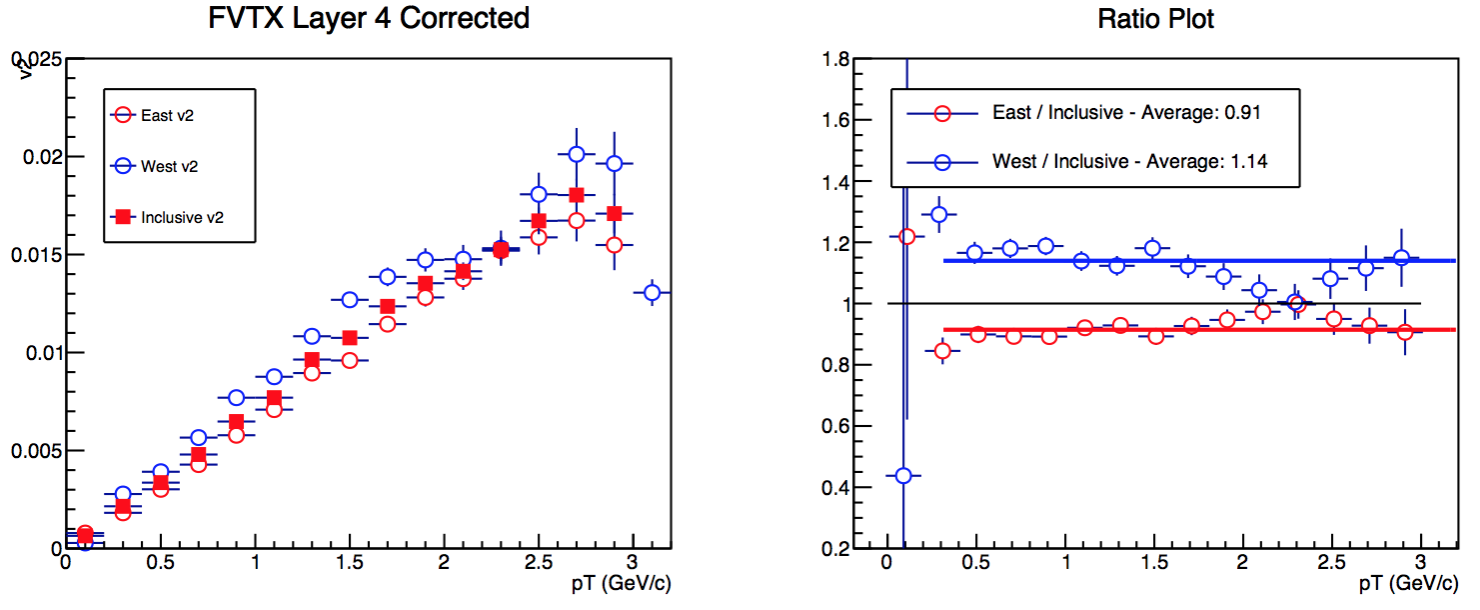
\includegraphics[width=0.65\linewidth]{figs/fvtx_4_data_cut.png}
\caption{FVTXS event plane measurement with inverse $\phi$ weighting and a 20\% cut and FVTX layer 4 of $v_{2}(\pt)$ with the  for the \pau \sqsn = 200 GeV (left) and the ratio of the east and west $v_2$ measurements to the inclusive $v_2$ (right).}
\end{figure}

\begin{figure}

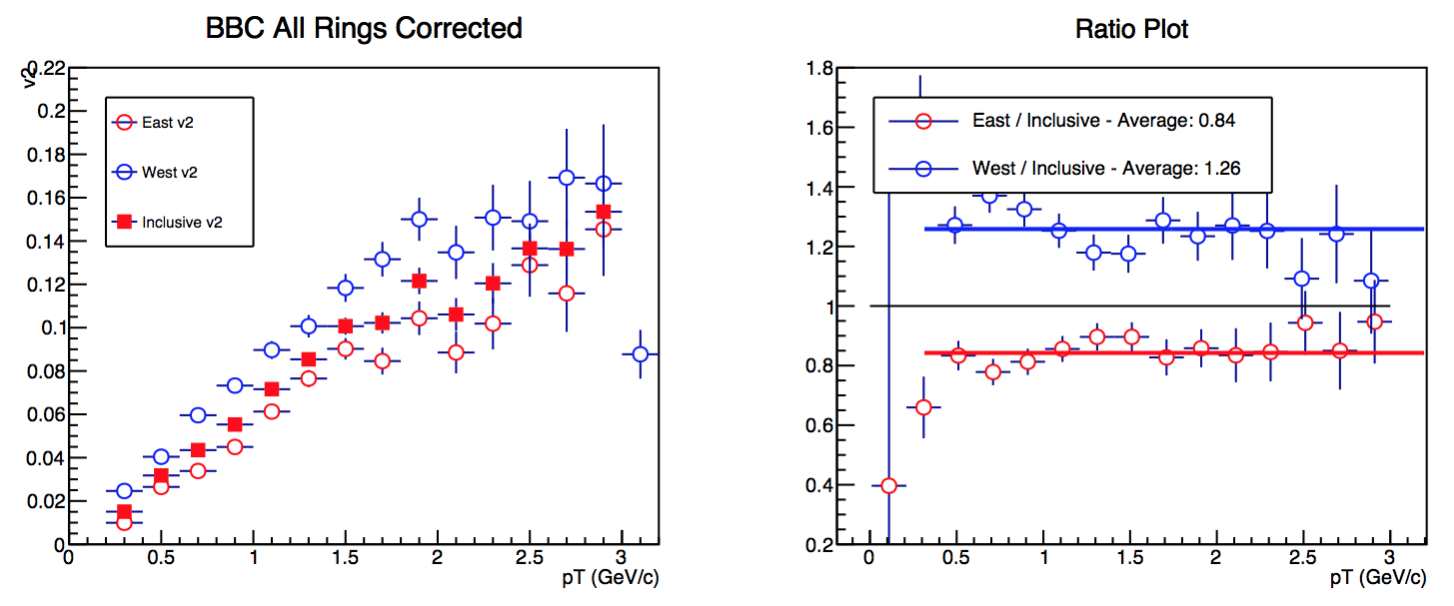
\includegraphics[width=0.65\linewidth]{figs/bbc_all_default.png}
\caption{BBCS event plane measurement with default correction and all BBC rings of $v_{2}(\pt)$ with the  for the \pau \sqsn = 200 GeV (left) and the ratio of the east and west $v_2$ measurements to the inclusive $v_2$ (right).}
\end{figure}

\begin{figure}

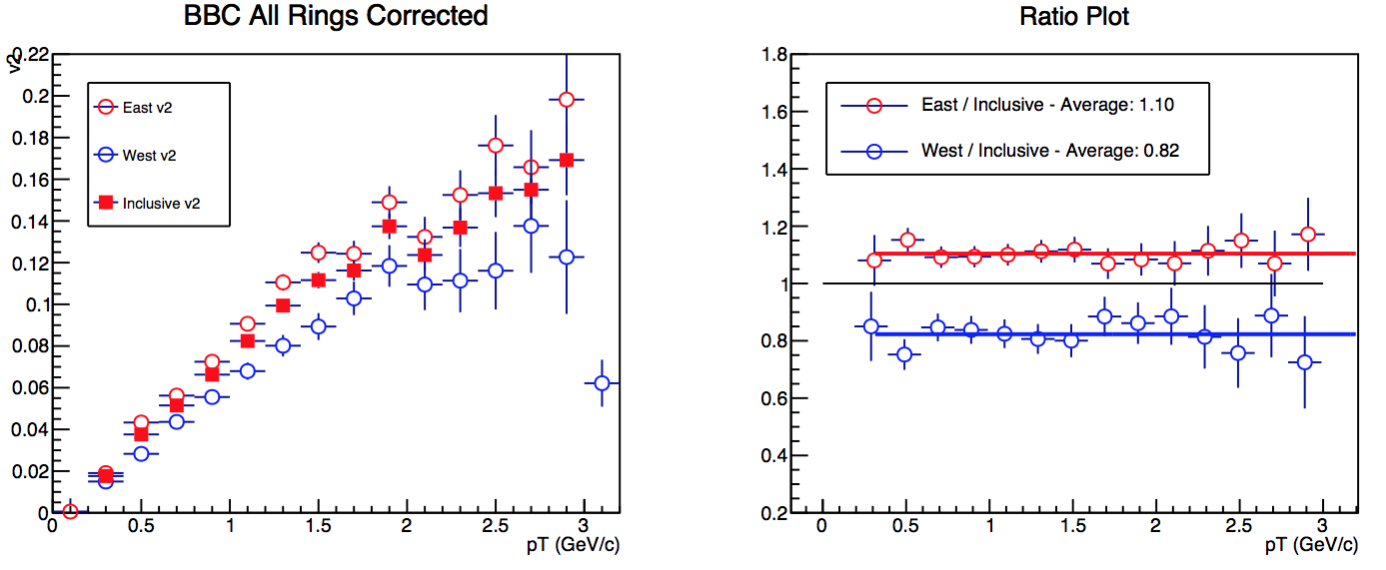
\includegraphics[width=0.65\linewidth]{figs/bbc_all_data.png}
\caption{BBCS event plane measurement with inverse charge correction and all BBC rings of $v_{2}(\pt)$ with the  for the \pau \sqsn = 200 GeV (left) and the ratio of the east and west $v_2$ measurements to the inclusive $v_2$ (right).}
\end{figure}

\begin{figure}
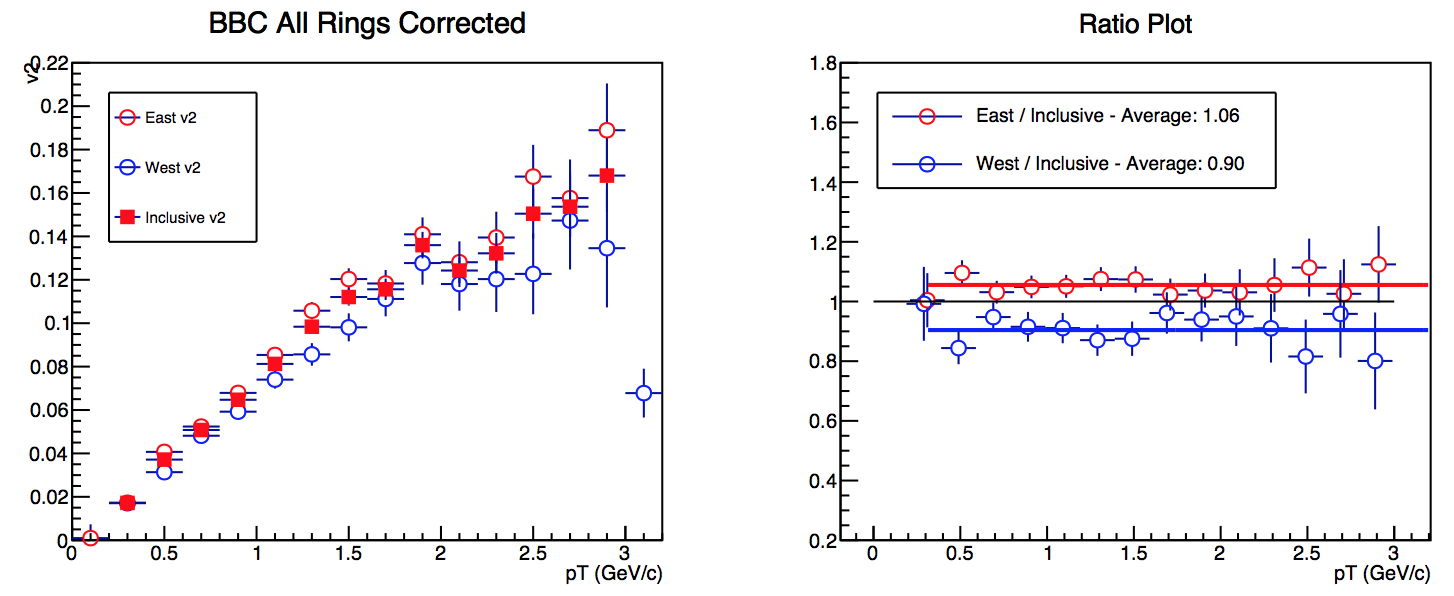
\includegraphics[width=0.65\linewidth]{figs/bbc_all_pp.png}
\caption{BBCS event plane measurement with \pp/\pau ratio correction and all BBC rings of $v_{2}(\pt)$ with the  for the \pau \sqsn = 200 GeV (left) and the ratio of the east and west $v_2$ measurements to the inclusive $v_2$ (right).}
\end{figure}

\begin{figure}
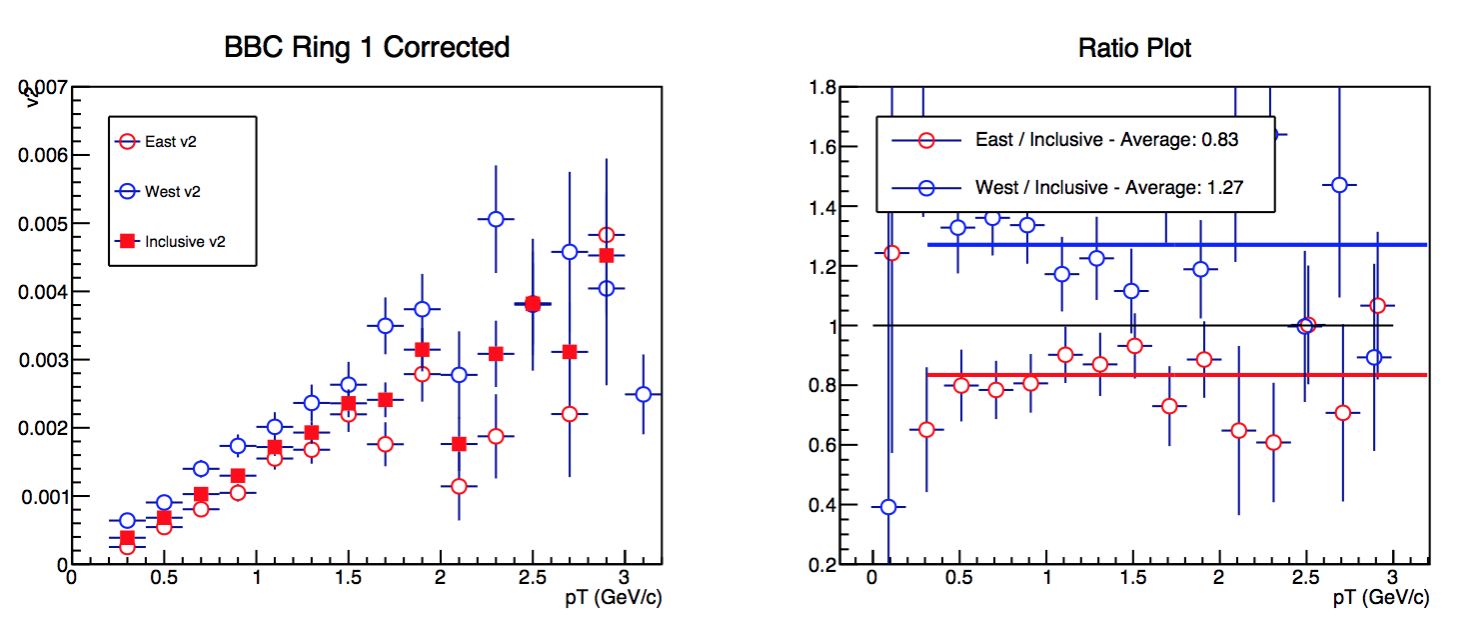
\includegraphics[width=0.65\linewidth]{figs/bbc_1_default.png}
\caption{BBCS event plane measurement with default correction and BBC ring 1 of $v_{2}(\pt)$ with the  for the \pau \sqsn = 200 GeV (left) and the ratio of the east and west $v_2$ measurements to the inclusive $v_2$ (right).}
\end{figure}

\begin{figure}
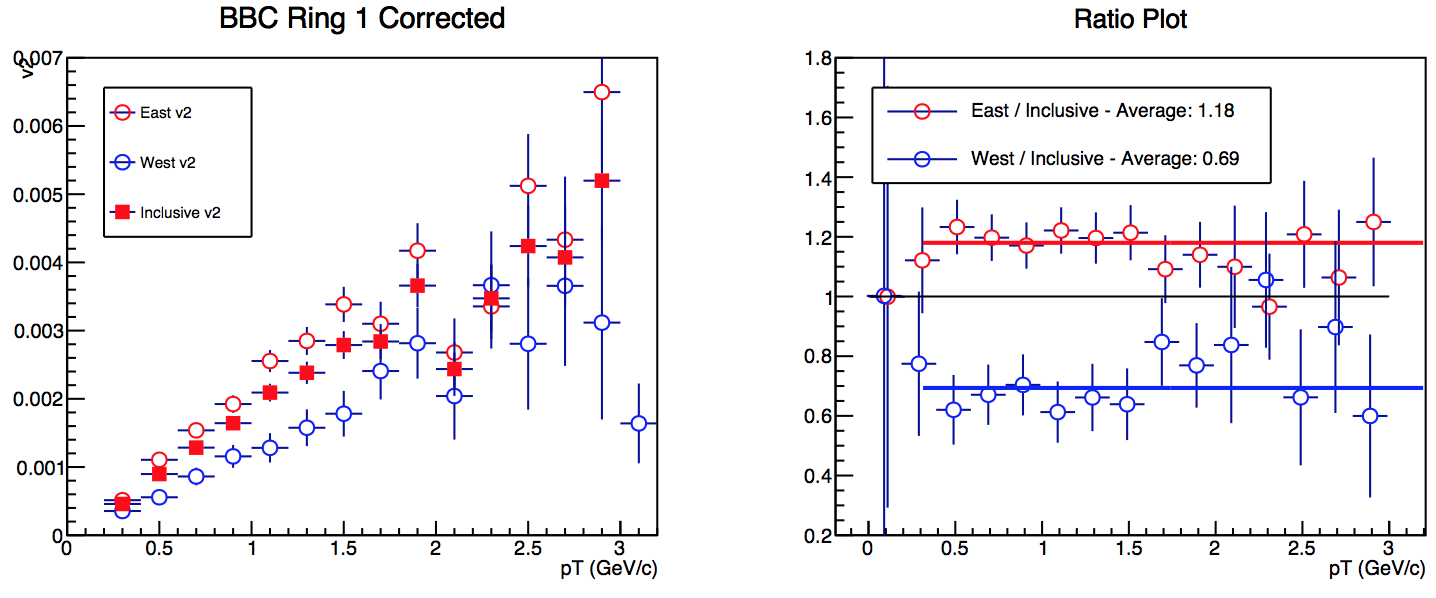
\includegraphics[width=0.65\linewidth]{figs/bbc_1_data.png}
\caption{BBCS event plane measurement with inverse charge correction and BBC ring 1 of $v_{2}(\pt)$ with the  for the \pau \sqsn = 200 GeV (left) and the ratio of the east and west $v_2$ measurements to the inclusive $v_2$ (right).}
\end{figure}
\clearpage
\begin{figure}
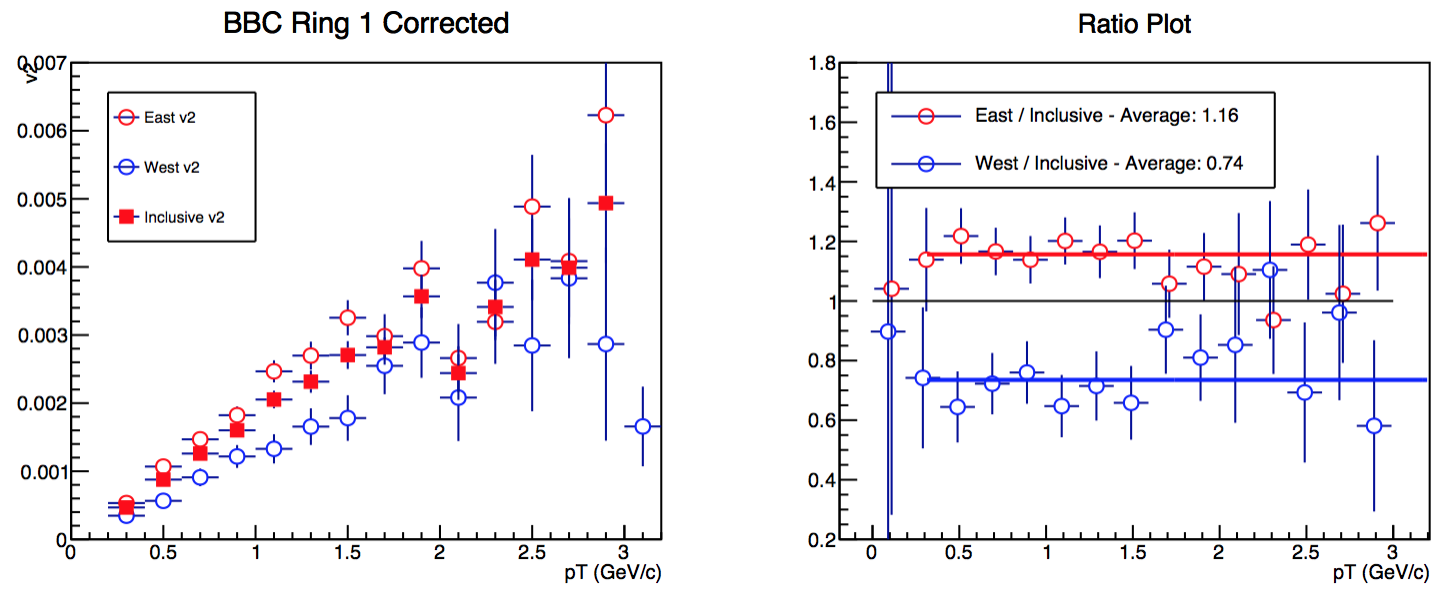
\includegraphics[width=0.65\linewidth]{figs/bbc_1_pp.png}
\caption{BBCS event plane measurement with \pp/\pau ratio correction and BBC ring 1 of $v_{2}(\pt)$ with the  for the \pau \sqsn = 200 GeV (left) and the ratio of the east and west $v_2$ measurements to the inclusive $v_2$ (right).}
\end{figure}

\begin{figure}

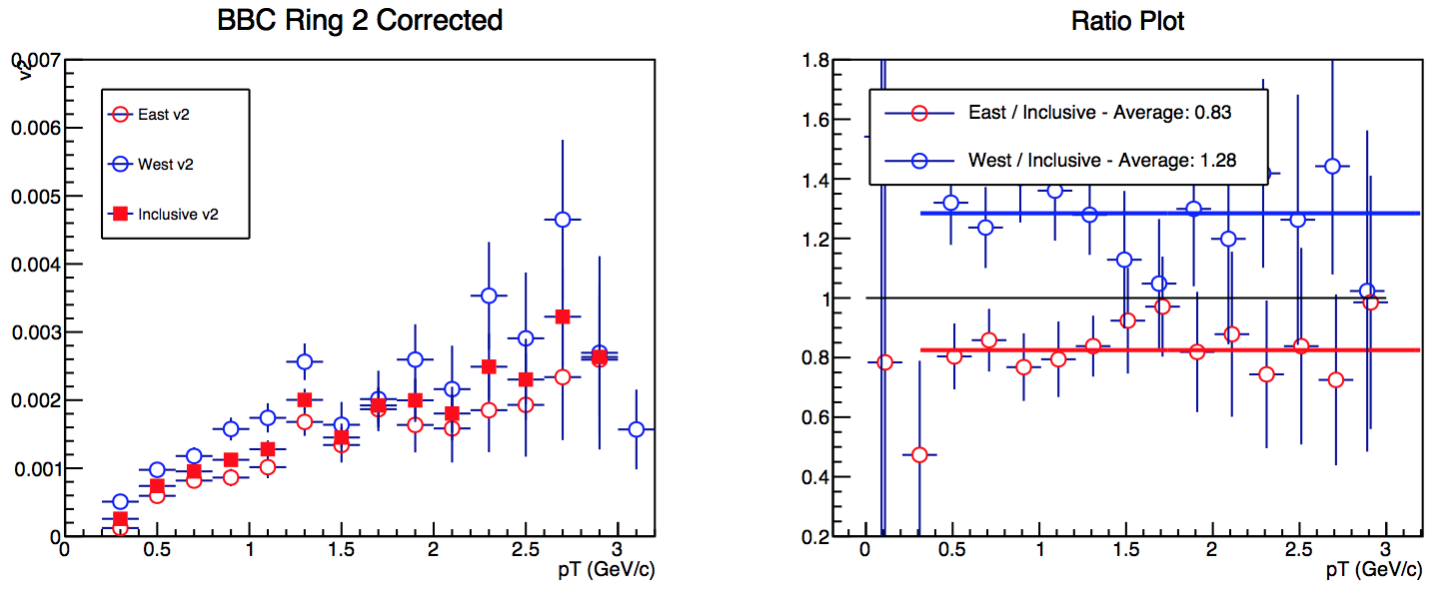
\includegraphics[width=0.65\linewidth]{figs/bbc_2_default.png}
\caption{BBCS event plane measurement with default correction and BBC ring 2 of $v_{2}(\pt)$ with the  for the \pau \sqsn = 200 GeV (left) and the ratio of the east and west $v_2$ measurements to the inclusive $v_2$ (right).}
\end{figure}

\begin{figure}

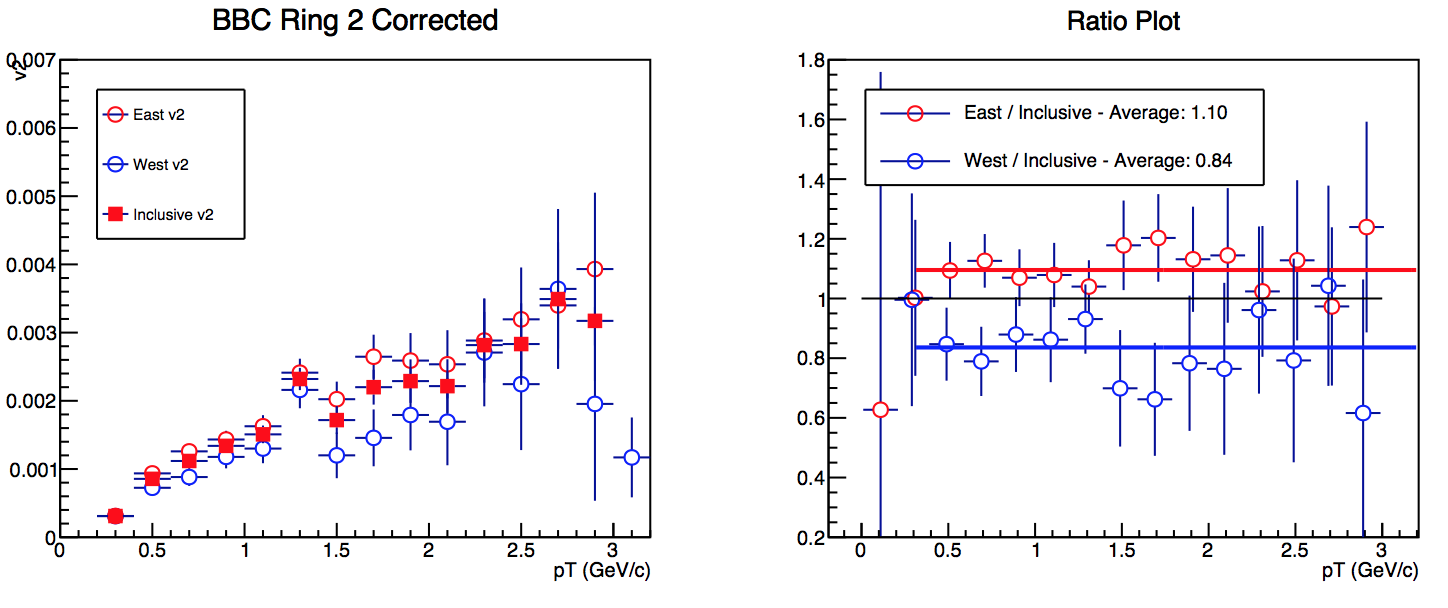
\includegraphics[width=0.65\linewidth]{figs/bbc_2_data.png}
\caption{BBCS event plane measurement with inverse charge correction and BBC ring 2 of $v_{2}(\pt)$ with the  for the \pau \sqsn = 200 GeV (left) and the ratio of the east and west $v_2$ measurements to the inclusive $v_2$ (right).}
\end{figure}

\begin{figure}

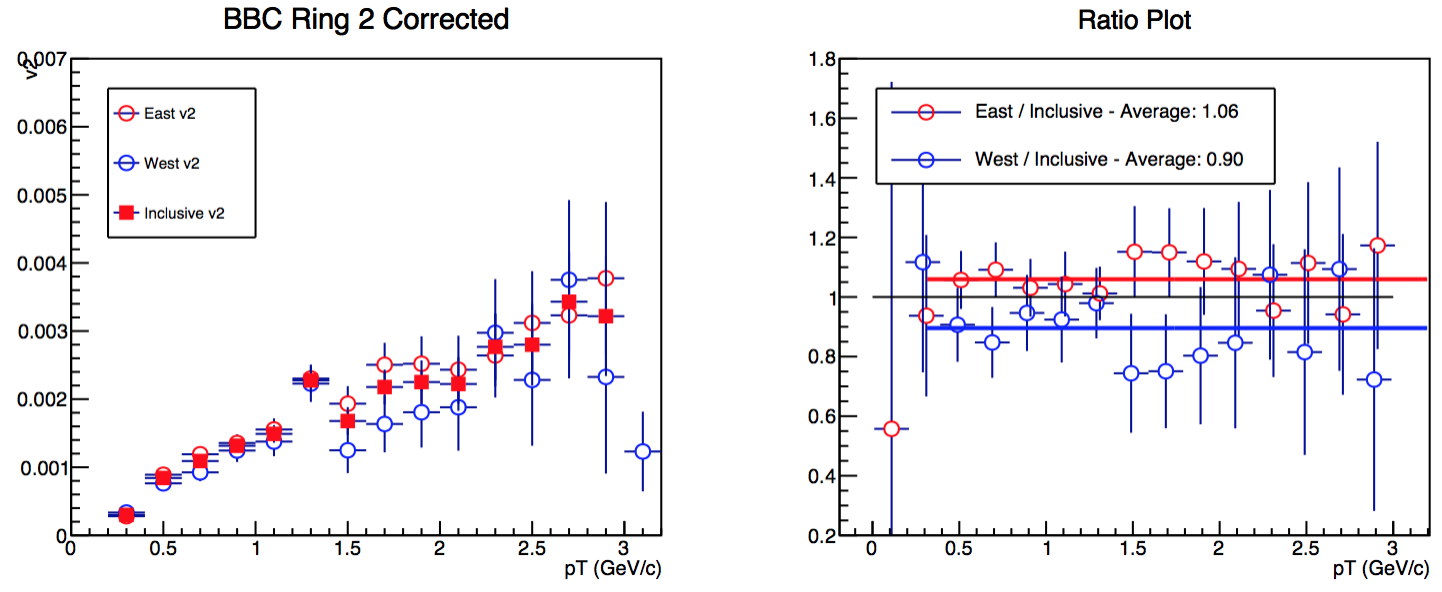
\includegraphics[width=0.65\linewidth]{figs/bbc_2_pp.png}
\caption{BBCS event plane measurement with \pp/\pau ratio correction and BBC ring 2 of $v_{2}(\pt)$ with the  for the \pau \sqsn = 200 GeV (left) and the ratio of the east and west $v_2$ measurements to the inclusive $v_2$ (right).}
\end{figure}

\begin{figure}

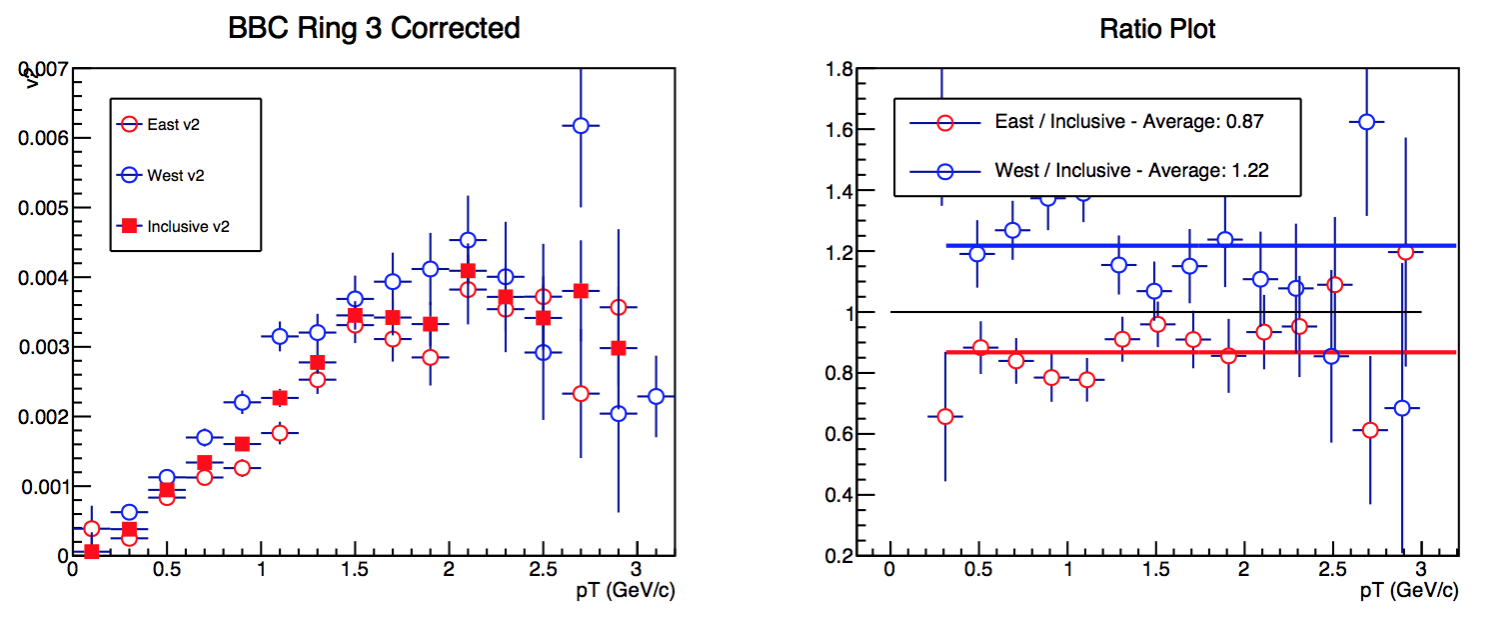
\includegraphics[width=0.65\linewidth]{figs/bbc_3_default.png}
\caption{BBCS event plane measurement with default correction and BBC ring 3 of $v_{2}(\pt)$ with the  for the \pau \sqsn = 200 GeV (left) and the ratio of the east and west $v_2$ measurements to the inclusive $v_2$ (right).}
\end{figure}

\begin{figure}
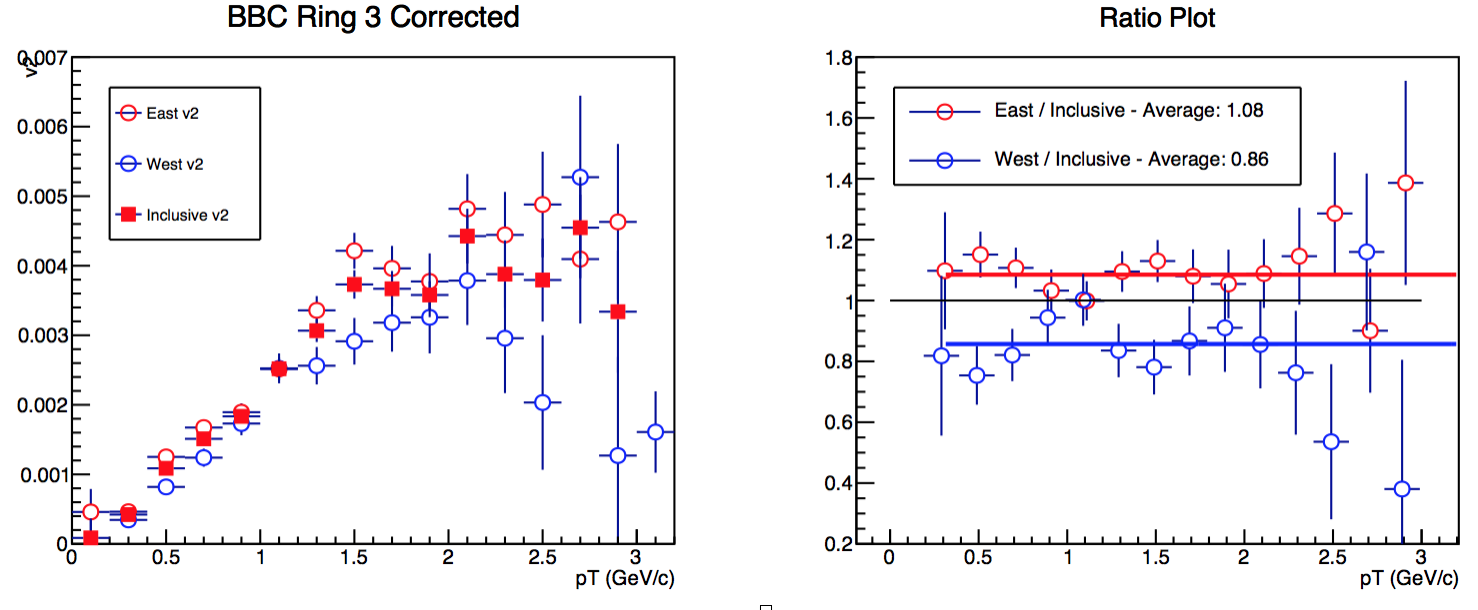
\includegraphics[width=0.65\linewidth]{figs/bbc_3_data.png}
\caption{BBCS event plane measurement with inverse charge correction and BBC ring 3 of $v_{2}(\pt)$ with the  for the \pau \sqsn = 200 GeV (left) and the ratio of the east and west $v_2$ measurements to the inclusive $v_2$ (right).}
\end{figure}

\begin{figure}
\centering
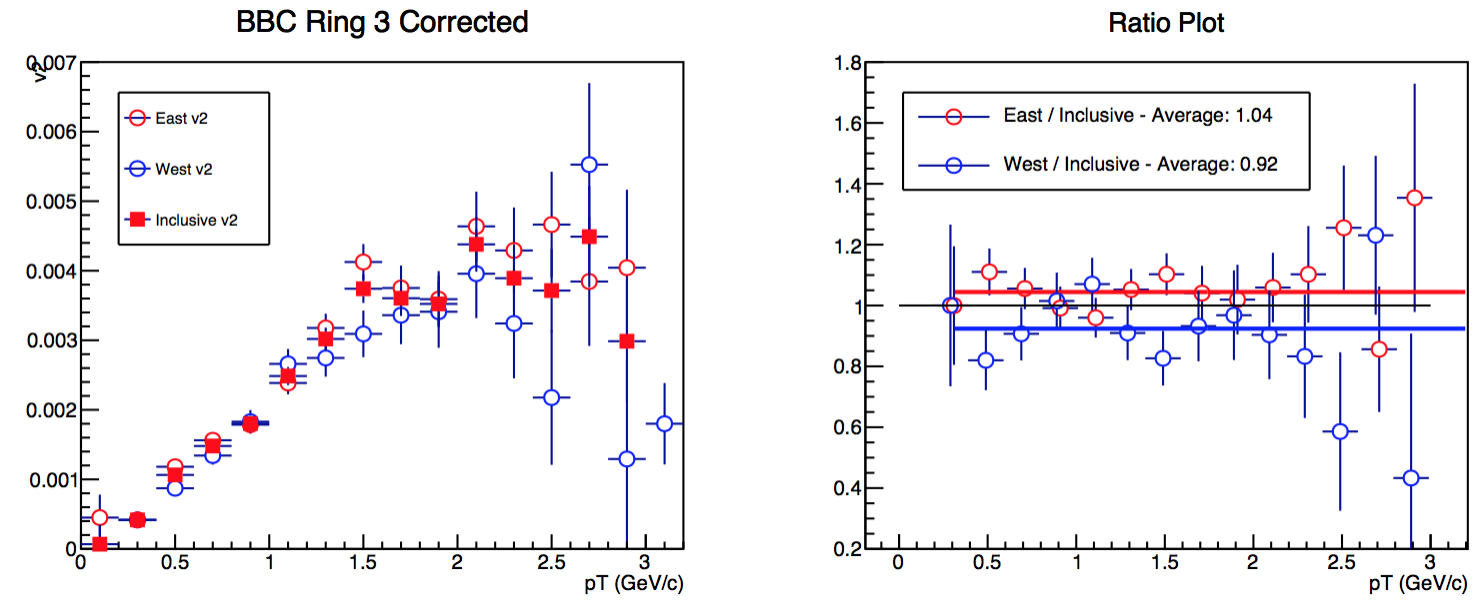
\includegraphics[width=0.65\linewidth]{figs/bbc_3_pp.png}
\caption{BBCS event plane measurement with \pp/\pau ratio correction and BBC ring 3 of $v_{2}(\pt)$ with the  for the \pau \sqsn = 200 GeV (left) and the ratio of the east and west $v_2$ measurements to the inclusive $v_2$ (right).}
\end{figure}
\clearpage
\begin{figure}
\centering
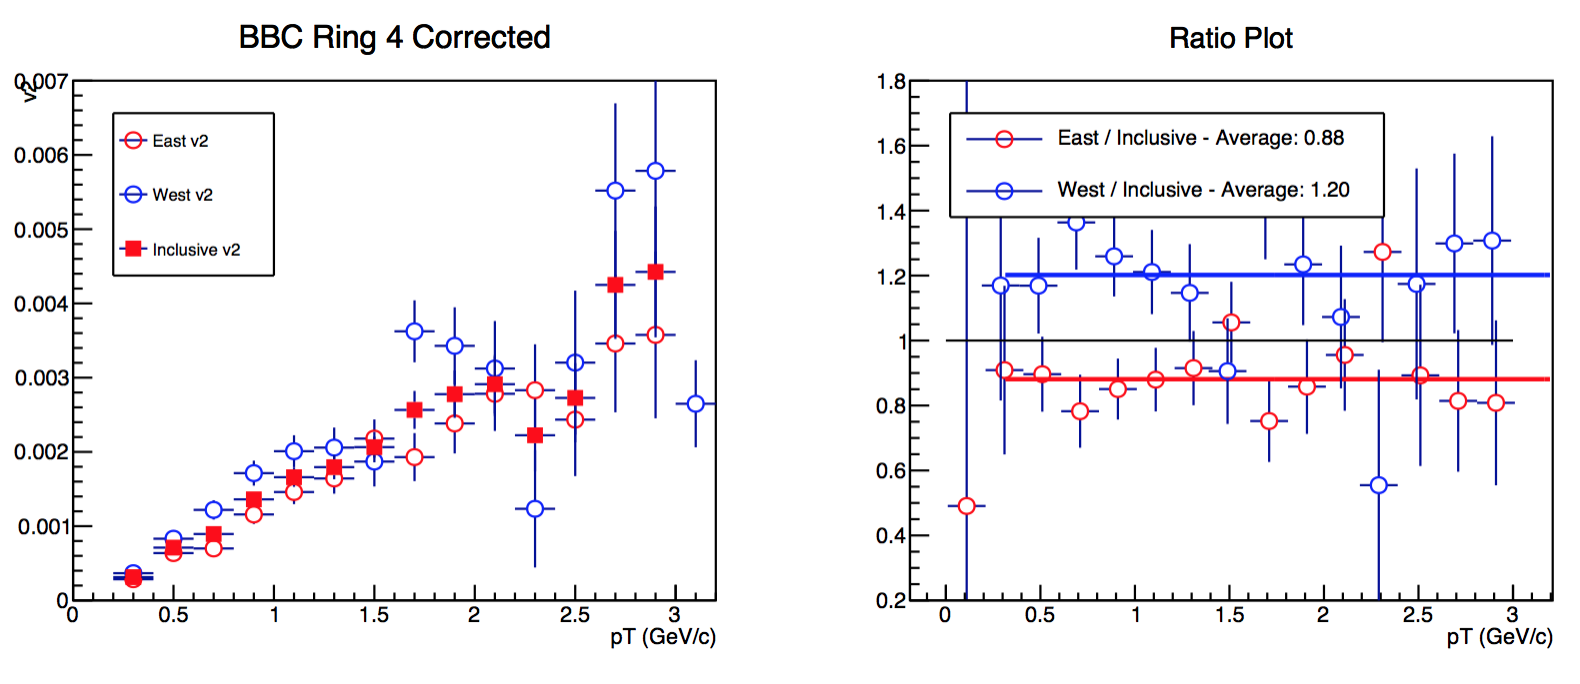
\includegraphics[width=0.65\linewidth]{figs/bbc_4_default.png}
\caption{BBCS event plane measurement with default correction and BBC ring 4 of $v_{2}(\pt)$ with the  for the \pau \sqsn = 200 GeV (left) and the ratio of the east and west $v_2$ measurements to the inclusive $v_2$ (right).}
\end{figure}

\begin{figure}
\centering
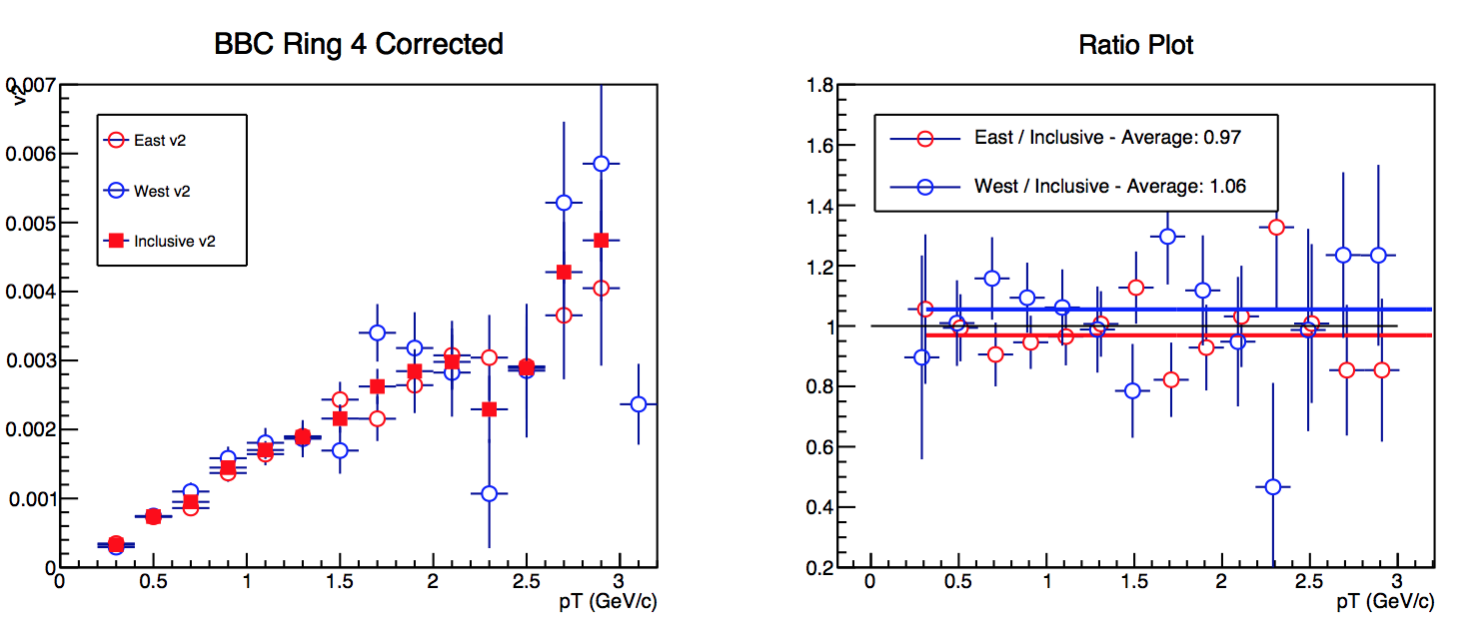
\includegraphics[width=0.65\linewidth]{figs/bbc_4_data.png}
\caption{BBCS event plane measurement with inverse charge correction and BBC ring 4 of $v_{2}(\pt)$ with the  for the \pau \sqsn = 200 GeV (left) and the ratio of the east and west $v_2$ measurements to the inclusive $v_2$ (right).}
\end{figure}

\begin{figure}
\centering
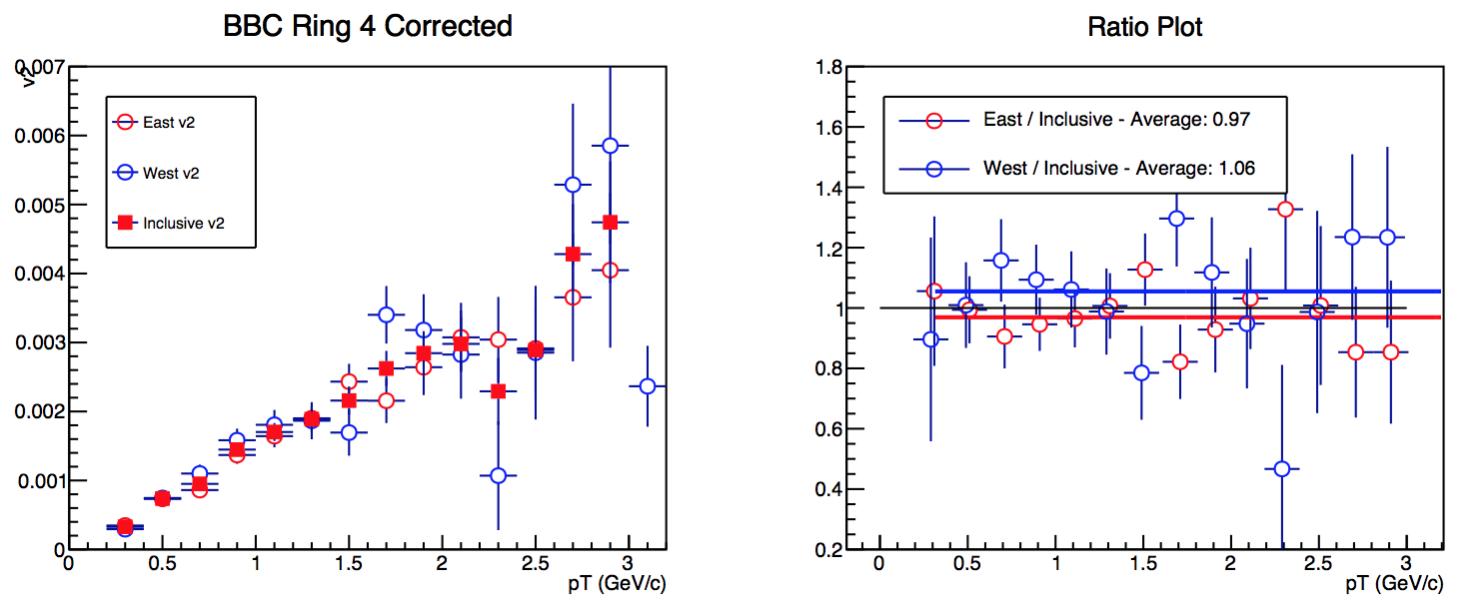
\includegraphics[width=0.65\linewidth]{figs/bbc_4_pp.png}
\caption{BBCS event plane measurement with \pp/\pau ratio correction and BBC ring 4 of $v_{2}(\pt)$ with the  for the \pau \sqsn = 200 GeV (left) and the ratio of the east and west $v_2$ measurements to the inclusive $v_2$ (right).}
\end{figure}

\begin{figure}
\centering
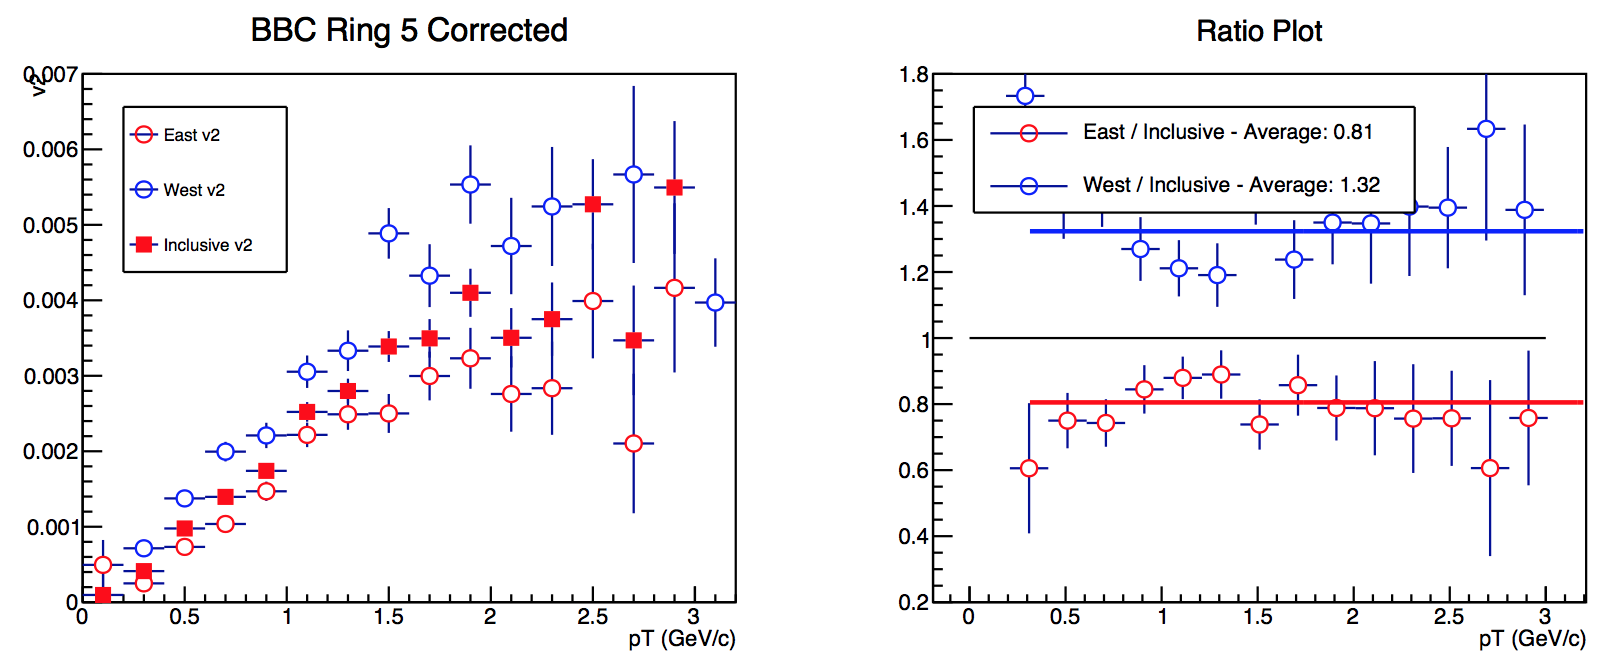
\includegraphics[width=0.65\linewidth]{figs/bbc_5_default.png}
\caption{BBCS event plane measurement with default correction and BBC ring 5 of $v_{2}(\pt)$ with the  for the \pau \sqsn = 200 GeV (left) and the ratio of the east and west $v_2$ measurements to the inclusive $v_2$ (right).}
\end{figure}

\begin{figure}
\centering
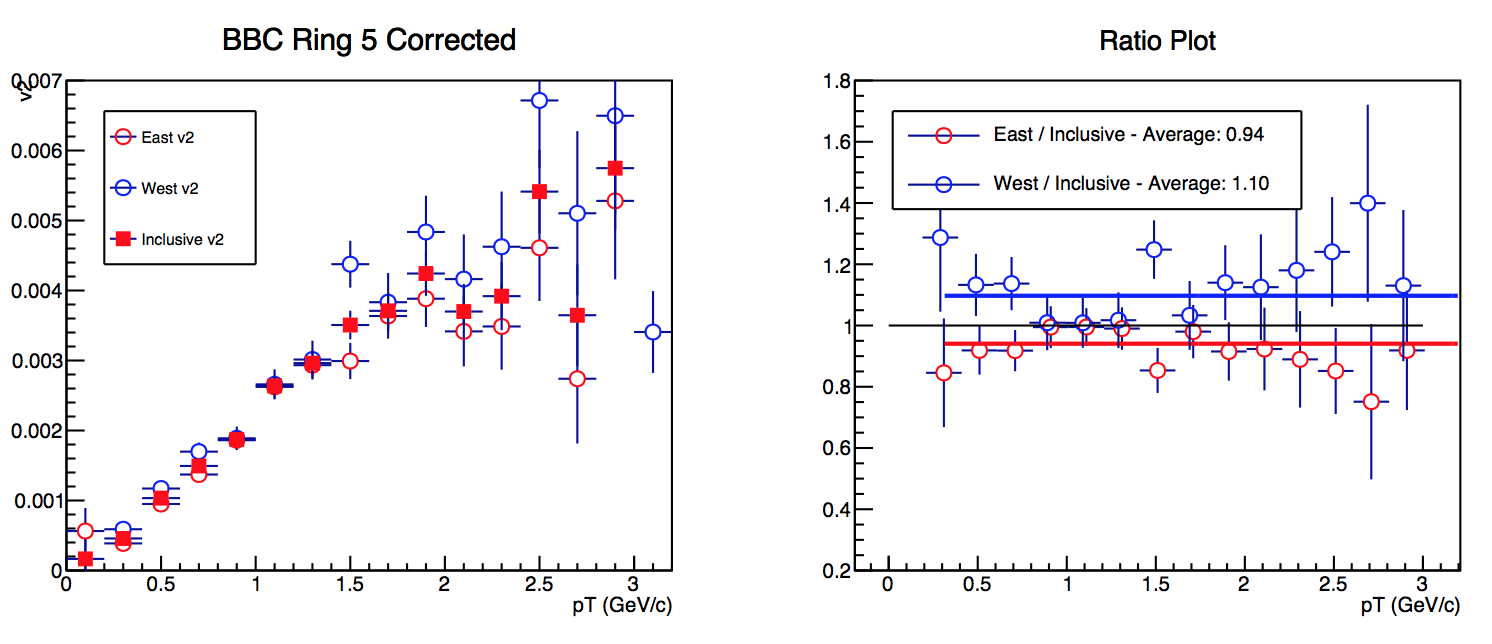
\includegraphics[width=0.65\linewidth]{figs/bbc_5_data.png}
\caption{BBCS event plane measurement with inverse charge correction and BBC ring 5 of $v_{2}(\pt)$ with the  for the \pau \sqsn = 200 GeV (left) and the ratio of the east and west $v_2$ measurements to the inclusive $v_2$ (right).}
\end{figure}

\begin{figure}
\centering
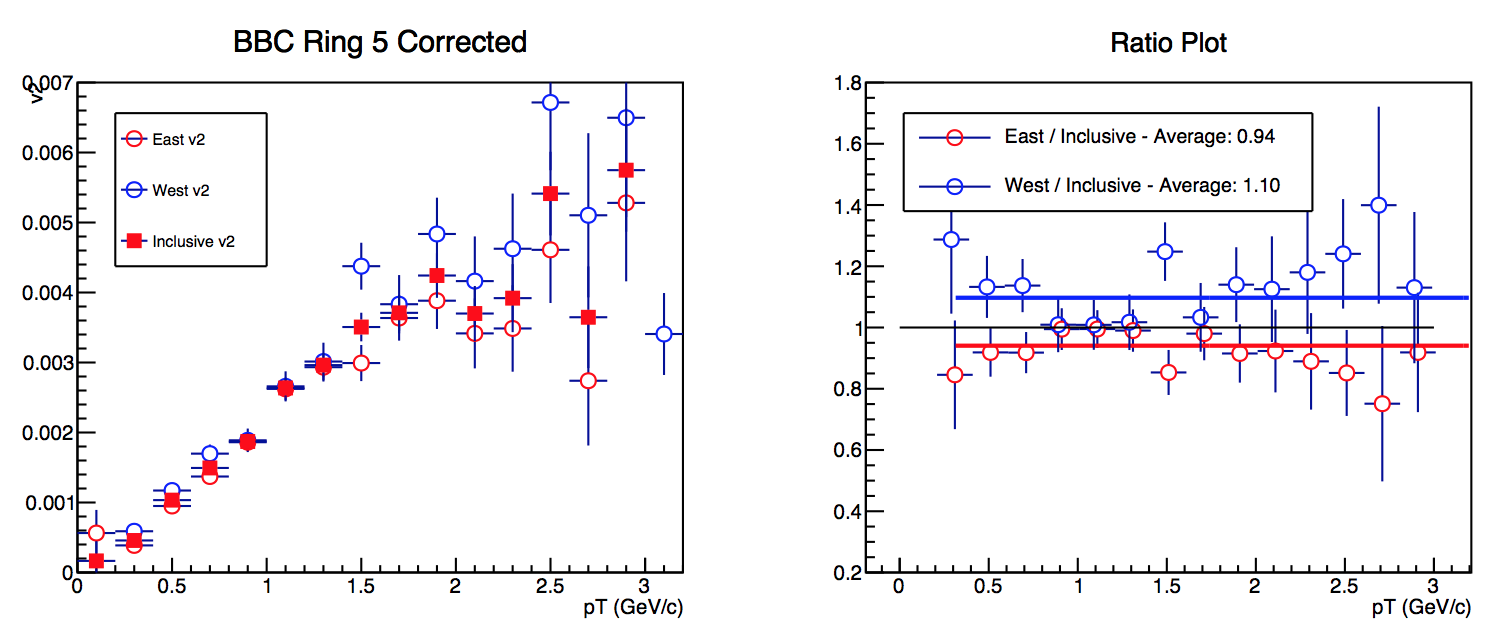
\includegraphics[width=0.65\linewidth]{figs/bbc_5_pp.png}
\caption{BBCS event plane measurement with \pp/\pau ratio correction and BBC ring 5 of $v_{2}(\pt)$ with the  for the \pau \sqsn = 200 GeV (left) and the ratio of the east and west $v_2$ measurements to the inclusive $v_2$ (right).}
\end{figure}
